\documentclass[a4paper,12pt]{article}

%Class
	%\documentclass[a4paper,12pt]{article}

%Packages
	\usepackage{amsmath}					% Standard maths
	\usepackage{amssymb}					% Standard maths
	\usepackage{amsthm}						% Standard maths
	\usepackage{thmtools, thm-restate}% Theorem styles
	\usepackage{mathtools}
	\usepackage[newzealand]{babel}% Date/time in British format (yes, I know it says NZ)
	\usepackage{datetime}					% Date/time
	\usepackage{multirow}					% For stacked subscripts
	\usepackage{xcolor}						% For colour!
	\usepackage[normalem]{ulem}		% For strikeout
	\usepackage{isomath}
	\usepackage{fancyhdr}					% For the headers
	\usepackage{mfirstuc}					% For the headers
	\usepackage[hmargin=1in,top=0.8in,bottom=1in]{geometry} % Page margins more reasonable
	\usepackage{graphicx}					% For including graphics
	%\usepackage{float}						% For something
	\usepackage{enumitem}					% For numbering tweaks
	\usepackage{pgfplots}
	\usepackage[margin=15pt,font={footnotesize},labelfont=bf,format=hang]{caption}
\usepackage[margin=15pt,font={footnotesize},labelfont=bf,format=hang]{subcaption}
	\usepackage{url}
	\usepackage[hidelinks]{hyperref}	% For hyperlinks
	\usepackage{breakurl}
	\usepackage{cleveref}
	\usepackage[scaled=.92]{helvet}
	\newbool{show_question}
	\newbool{show_solution}
	\newcommand{\solutioninheading}{\ifbool{show_solution}{: SOLUTIONS}{}}
	\usepackage{pgfplots}
\newcommand{\ep}{\varepsilon}

\makeatletter 
\newcommand\mynobreakpar{\par\nobreak\@afterheading} 
\makeatother

    \newcommand{\question}[3]{
    	\item \textbf{#1} \mynobreakpar \nobreak \medskip % Title
    	%
    	\ifbool{show_question}{\nobreak#2}{} % Question
    	%
    	%
    	\ifbool{show_question}{\ifbool{show_solution}{\par\medskip\textbf{Solution:}}{}}{} % Both
    	\ifbool{show_solution}{#3}{} % Answer
    }			

%MATHEMATICAL SHORTCUTS
%Two and three-part definitions
	\newcommand{\twopartdef}[4]
	{	\left\{
			\begin{array}{ll}
				#1 & \mbox{if } #2 \\
				#3 & \mbox{if } #4
			\end{array}
		\right.}
%	\newcommand{\threepartdef}[6]
%	{	\left\{
%			\begin{array}{ll}
%				#1 & \mbox{if } #2 \\
%				#3 & \mbox{if } #4 \\
%				#5 & \mbox{if } #6
%			\end{array}
%		\right.}
%Blackboard bold	
	\newcommand{\N}{{\mathbb N}} 
	\newcommand{\R}{{\mathbb R}} 
	\newcommand{\C}{{\mathbb C}} 
	%Curly letters
%	\newcommand{\E}{{\mathcal E}}	
%	\newcommand{\F}{{\mathcal F}} 
%	\newcommand{\Null}{{\mathcal N}} 
%	\newcommand{\R}{\mathcal{R}} 
%	\newcommand{\Z}{\mathcal{Z}} 
%Uprights
	\newcommand{\D}{{\mathrm D}}
	\renewcommand{\d}{{\mathrm d}}
%Easy Greeks
%	\def\a{\alpha}
%	\def\g{\gamma}
%	\newcommand{\e}{{\varepsilon}}
%	\newcommand{\la}{{\lambda}}  
%	\newcommand{\om}{{\Omega}}
	\renewcommand{\epsilon}{\varepsilon}
	
%Vector operators
	\def \p {\partial}
	\newcommand{\del}{{\nabla}}
	\newcommand{\grad}{{\nabla}}
    \newcommand{\vdel}{\boldsymbol{\nabla}}
    \newcommand{\vgrad}{\boldsymbol{\nabla}}
    \newcommand{\vnabla}{\boldsymbol{\nabla}}
	\newcommand{\cross}{{\times}}
	\newcommand{\Lap}{{\nabla^2}} 
%Arrows
%	\newcommand{\goesto}[1]{\xrightarrow[#1]{}}
%hats
%	\newcommand{\nhat}{\widehat{\v{n}}}
%	\newcommand{\shat}{\widehat{\v{s}}}
	\renewcommand{\hat}{\widehat}
%Note to self
%	\newcommand{\note}[1]{[\textbf{\textsl{\MakeUppercase{#1}}}]}
	
%Stress tensor
%	\newcommand{\T}{\vg{\sigma}}

% Vectors, quaternions etc.
\renewcommand{\v}[1]{\mathbfit{#1}}      % Generic vector
\newcommand{\vc}[1]{\bm{\mathcal{#1}}}      % vector mathcal
\newcommand{\uv}[1]{\widehat{\mathbfit{#1}}}      % Generic unit vector
\newcommand{\q}[1]{\mathsfbfit{#1}}        % Generic quaternion
\renewcommand{\t}[1]{\mathsfbfit{#1}}	 % Generic tensor
\newcommand{\m}[1]{\mathsfbfit{#1}}	 % Generic matrix
\newcommand{\vu}[1]{\mathbf{#1}}         % Upright vector (for zero vector)
\newcommand{\qu}[1]{\mathbf{#1}}       % Upright quaternion (for zero quaternion)
\newcommand{\tu}[1]{\bm{\mathsf{#1}}}	 % Upright tensor (for zero tensor)

%Real and imaginary
\renewcommand{\Re}{\operatorname{Re}}
\renewcommand{\Im}{\operatorname{Im}}
	
%Non-dim numbers
%	\renewcommand{\Re}{\operatorname{Re}}
%	\newcommand{\Bi}{\operatorname{Bi}}
%	\newcommand{\Fo}{\operatorname{Fo}}
	
%Misc
\DeclareMathSymbol{\Delta}{\mathalpha}{operators}{1} % Keeps Delta upright
\DeclareMathSymbol{\Gamma}{\mathalpha}{operators}{0} % Keeps Gamma upright
	\newcommand{\cosec}{\operatorname{cosec}}
	\newcommand{\cosech}{\operatorname{cosech}}
	\newcommand{\sech}{\operatorname{sech}}
	\newcommand{\tr}{\operatorname{tr}}
	\newcommand{\erf}{\operatorname{erf}}
	\newcommand{\order}{\mathcal{O}}
%	\newcommand{\V}{\mathcal{V}} % 	CurlyV = (Bi V) / (1 + Bi)

% Differentiating 
\newcommand{\fd}[2]{\mathchoice{\frac{\d #1}{\d #2}}{\d #1/\d #2}{\d #1/\d #2}{\d #1/\d #2}}
\newcommand{\fdd}[2]{\mathchoice{\frac{\d^2 #1}{\d #2^2}}{\d^2 #1/\d #2^2}{\d^2 #1/\d #2^2}{\d^2 #1/\d #2^2}}
\newcommand{\fddd}[2]{\mathchoice{\frac{\d^3 #1}{\d #2^3}}{\d^3 #1/\d #2^3}{\d^3 #1/\d #2^3}{\d^3 #1/\d #2^3}}
\newcommand{\fdddd}[2]{\mathchoice{\frac{\d^4 #1}{\d #2^4}}{\d^4 #1/\d #2^4}{\d^4 #1/\d #2^4}{\d^4 #1/\d #2^4}}
\newcommand{\fdn}[3]{\mathchoice{\frac{\d^{#1} #2}{\d #3^{#1}}}{\d^{#1} #2/\d #3^{#1}}{\d^{#1} #2/\d #3^{#1}}{\d^{#1} #2/\d #3^{#1}}}
\newcommand{\pd}[2]{\mathchoice{\frac{\p #1}{\p #2}}{\p #1/\p #2}{\p #1/\p #2}{\p #1/\p #2}}
\newcommand{\pdd}[2]{\mathchoice{\frac{\p^2 #1}{\p #2^2}}{\p^2 #1/\p #2^2}{\p^2 #1/\p #2^2}{\p^2 #1/\p #2^2}}
\newcommand{\pddmixed}[3]{\frac{\p^2 #1}{\p #2 \p #3}}
\newcommand{\pddd}[2]{\frac{\p^3 #1}{\p #2^3}}
\newcommand{\pdn}[3]{\mathchoice{\frac{\p^{#1} #2}{\p #3^{#1}}}{\p^{#1} #2/\p #3^{#1}}{\p^{#1} #2/\p #3^{#1}}{\p^{#1} #2/\p #3^{#1}}}
	
	% Misc
\newcommand{\e}{\mathrm{e}}
\renewcommand{\i}{\mathrm{i}}
\newcommand{\dx}{\,\mathrm{d}x}
\newcommand{\dy}{\,\mathrm{d}y}
\renewcommand{\epsilon}{\varepsilon}
\renewcommand{\Re}{\operatorname{Re}}
\newcommand{\Four}{\mathcal{F}}

\newcommand{\mat}[4]{\begin{pmatrix}#1 & #2 \\ #3 & #4 \end{pmatrix}}

	%Column vectors
	\makeatletter
\newcommand\rcvector[2][\\]{\ensuremath{%
  \global\def\rc@delim{#1}%
    \negthinspace\begin{pmatrix}
      \rc@vector #2,\relax\noexpand\@eolst%
    \end{pmatrix}}}
\def\rc@vector #1,#2\@eolst{%
  \ifx\relax#2\relax
    #1
  \else
    #1\rc@delim
    \rc@vector #2\@eolst%
  \fi}
\makeatother

\newcommand{\colvec}{\rcvector}
\newcommand{\rowvec}{\rcvector}
\renewcommand{\binom}{\rcvector}
	
	%Colours
%	\newcommand{\orange}[1]{{\color{orange} #1 }}
%	\newcommand{\blue}[1]{{\color{blue} #1 }}

%Theorem styles
%	\declaretheoremstyle[headpunct={\:\:\:}, shaded={bgcolor={rgb}{0.9,0.9,0.9}, margin=5pt}]{problem}
%	\declaretheoremstyle[headpunct={\:\:\:}, shaded={rulecolor=black, rulewidth=0.4pt, bgcolor={rgb}{1,1,1}, margin=5pt}]{definition}
%	\declaretheoremstyle[headpunct={\:\:\:}, spaceabove=15pt, notefont=\bf, notebraces={(}{)}]{theorem}
%	\declaretheoremstyle[headpunct={\:\:\:}, numbered=no, spaceabove=15pt, qed={\checkmark}]{solution}
%	
%	\declaretheorem[style=definition,numberwithin=section]{definition}
%	\declaretheorem[numberlike=definition, style=theorem]{theorem}
%	\declaretheorem[numberlike=definition, style=theorem]{lemma}
%	\declaretheorem[numberlike=definition,style=problem]{problem}
%	\declaretheorem[numberlike=definition, style=theorem]{proposition}
%	\declaretheorem[numberlike=definition, style=theorem]{corollary}
%	\declaretheorem[numberlike=definition, style=theorem]{remark}
%	\declaretheorem[numberlike=definition, style=theorem]{example}
%	\declaretheorem[numberlike=definition, style=theorem]{notation}
%	\declaretheorem[style=solution]{solution}

%Depth of display breaks to allow	
	\allowdisplaybreaks[1]

%How deep do we want the Table of Contents to go?	
%	\setcounter{tocdepth}{1}

%Sections
\makeatletter
\renewcommand{\section}{\@startsection
{section}%                   % the name
{1}%                         % the level
{0mm}%                       % the indent
{-\baselineskip}%            % the before skip
{0.5\baselineskip}%          % the after skip
{\normalfont\bfseries}} % the style
\makeatother

% Wavy underline
\makeatletter
\font\sixly=lasyb10 scaled 1200
\def\tinners{\bgroup \markoverwith{\lower8.5\p@\hbox{\sixly \char58}}\ULon}
\makeatother
\newcommand{\answer}[1]{\tinners{\; #1 \;}}

%Setting the footnotes to use *,**,+ etc rather than 1,2,3	
\renewcommand{\thefootnote}{\fnsymbol{footnote}}

%Italic quote environment
%\newenvironment{quoteitalic}{\begin{quote}\itshape}{\end{quote}}

%Heading
\newcommand{\heading}[2]{
\setlength{\parindent}{0pt}
\textbf{MATH3171 (Mathematical Biology III)}

\textbf{YEAR 2025--26, \MakeUppercase{#1} TERM}
\setlength{\parskip}{3ex}

\textbf{\MakeUppercase{#2}}
%
\setlength{\parskip}{2ex}

}

%========================================================================================================================
%DOCUMENT BEGINS HERE!

\setbool{show_question}{true}
\setbool{show_solution}{false}
\begin{document}
%
\heading{Michaelmas}{Problems class 1\solutioninheading}

\begin{enumerate}[label={\bf \arabic{*}.\;}, ref={\arabic{*}},itemsep=3ex, left=0ex]

    \question{A simple epidemic model}
    { % Question
      Consider a population which is either susceptible ($S$) or infected ($I$) with a disease.
      \begin{enumerate}[label=(\alph*)]
        \item We assume that the total population, $N$, is constant. Given the population is either susceptible or infected, write down a simple equation for $N$.
        \item Infected people infect susceptible people by interacting with them. By considering how we represented interactions between greenflies and ladybirds, write down an equation for $\fd{I}{t}$ in terms of $I$ and $S$.
        \item By substituting in $N$, eliminate $S$ from this equation and show that
        \begin{equation}
        	\fd{I}{t} = \beta I (N-I).
        \end{equation}
        Do you recognise this type of model from chapter 1?
        \item Find the equilibria of this model for $I$, establish when they are permissible, and assess their stability. You can assess the stability either graphically, or by doing an algebraic linear stability analysis (with $\ep$ etc.)
        \item What does this mean for the spread of the disease? 
      \end{enumerate}
    }
    { % Solution
      \begin{enumerate}[label=(\alph*)]
        \item $N = S + I$
        \item $\fd{I}{t} = \beta I S$, where $\beta > 0$.
        \item $\fd{I}{t} = \beta I (N-I)$. This is a logistic model.
        \item The equilibria are where $\fd{I}{t} = 0$, i.e.\ $I=0,N$ (no-one or everyone).

          To assess their stability, we can use two methods.
          \paragraph{Method I: Graphical analysis}
          Graphical analysis of the phase plane is really convenient, but often it requires us to make assumptions about the signs of our constants which we have to be careful to be explicit about. This isn't something to catch you out! Look here, where we've plotted the phase plane ($\fd{I}{t}$ against $I$):

          \begin{center}%
            %% Creator: Matplotlib, PGF backend
%%
%% To include the figure in your LaTeX document, write
%%   \input{<filename>.pgf}
%%
%% Make sure the required packages are loaded in your preamble
%%   \usepackage{pgf}
%%
%% and, on pdftex
%%   \usepackage[utf8]{inputenc}\DeclareUnicodeCharacter{2212}{-}
%%
%% or, on luatex and xetex
%%   \usepackage{unicode-math}
%%
%% Figures using additional raster images can only be included by \input if
%% they are in the same directory as the main LaTeX file. For loading figures
%% from other directories you can use the `import` package
%%   \usepackage{import}
%%
%% and then include the figures with
%%   \import{<path to file>}{<filename>.pgf}
%%
%% Matplotlib used the following preamble
%%   \usepackage{fontspec}
%%   \setmainfont{DejaVuSerif.ttf}[Path=/Users/adam/opt/anaconda3/lib/python3.8/site-packages/matplotlib/mpl-data/fonts/ttf/]
%%   \setsansfont{DejaVuSans.ttf}[Path=/Users/adam/opt/anaconda3/lib/python3.8/site-packages/matplotlib/mpl-data/fonts/ttf/]
%%   \setmonofont{DejaVuSansMono.ttf}[Path=/Users/adam/opt/anaconda3/lib/python3.8/site-packages/matplotlib/mpl-data/fonts/ttf/]
%%
\begingroup%
\makeatletter%
\begin{pgfpicture}%
\pgfpathrectangle{\pgfpointorigin}{\pgfqpoint{3.000000in}{2.200000in}}%
\pgfusepath{use as bounding box, clip}%
\begin{pgfscope}%
\pgfsetbuttcap%
\pgfsetmiterjoin%
\definecolor{currentfill}{rgb}{1.000000,1.000000,1.000000}%
\pgfsetfillcolor{currentfill}%
\pgfsetlinewidth{0.000000pt}%
\definecolor{currentstroke}{rgb}{1.000000,1.000000,1.000000}%
\pgfsetstrokecolor{currentstroke}%
\pgfsetdash{}{0pt}%
\pgfpathmoveto{\pgfqpoint{0.000000in}{0.000000in}}%
\pgfpathlineto{\pgfqpoint{3.000000in}{0.000000in}}%
\pgfpathlineto{\pgfqpoint{3.000000in}{2.200000in}}%
\pgfpathlineto{\pgfqpoint{0.000000in}{2.200000in}}%
\pgfpathclose%
\pgfusepath{fill}%
\end{pgfscope}%
\begin{pgfscope}%
\pgfsetbuttcap%
\pgfsetmiterjoin%
\definecolor{currentfill}{rgb}{1.000000,1.000000,1.000000}%
\pgfsetfillcolor{currentfill}%
\pgfsetlinewidth{0.000000pt}%
\definecolor{currentstroke}{rgb}{0.000000,0.000000,0.000000}%
\pgfsetstrokecolor{currentstroke}%
\pgfsetstrokeopacity{0.000000}%
\pgfsetdash{}{0pt}%
\pgfpathmoveto{\pgfqpoint{0.305640in}{0.033333in}}%
\pgfpathlineto{\pgfqpoint{2.966667in}{0.033333in}}%
\pgfpathlineto{\pgfqpoint{2.966667in}{2.166667in}}%
\pgfpathlineto{\pgfqpoint{0.305640in}{2.166667in}}%
\pgfpathclose%
\pgfusepath{fill}%
\end{pgfscope}%
\begin{pgfscope}%
\pgfsetroundcap%
\pgfsetroundjoin%
\pgfsetlinewidth{0.602250pt}%
\definecolor{currentstroke}{rgb}{0.172549,0.627451,0.172549}%
\pgfsetstrokecolor{currentstroke}%
\pgfsetdash{}{0pt}%
\pgfpathmoveto{\pgfqpoint{1.093707in}{1.471119in}}%
\pgfpathquadraticcurveto{\pgfqpoint{1.256010in}{1.471119in}}{\pgfqpoint{1.408997in}{1.471119in}}%
\pgfusepath{stroke}%
\end{pgfscope}%
\begin{pgfscope}%
\pgfsetroundcap%
\pgfsetroundjoin%
\pgfsetlinewidth{0.602250pt}%
\definecolor{currentstroke}{rgb}{0.172549,0.627451,0.172549}%
\pgfsetstrokecolor{currentstroke}%
\pgfsetdash{}{0pt}%
\pgfpathmoveto{\pgfqpoint{1.342331in}{1.504452in}}%
\pgfpathlineto{\pgfqpoint{1.408997in}{1.471119in}}%
\pgfpathlineto{\pgfqpoint{1.342331in}{1.437785in}}%
\pgfusepath{stroke}%
\end{pgfscope}%
\begin{pgfscope}%
\pgfsetroundcap%
\pgfsetroundjoin%
\pgfsetlinewidth{0.602250pt}%
\definecolor{currentstroke}{rgb}{0.172549,0.627451,0.172549}%
\pgfsetstrokecolor{currentstroke}%
\pgfsetdash{}{0pt}%
\pgfpathmoveto{\pgfqpoint{2.938894in}{1.471119in}}%
\pgfpathquadraticcurveto{\pgfqpoint{2.776590in}{1.471119in}}{\pgfqpoint{2.623603in}{1.471119in}}%
\pgfusepath{stroke}%
\end{pgfscope}%
\begin{pgfscope}%
\pgfsetroundcap%
\pgfsetroundjoin%
\pgfsetlinewidth{0.602250pt}%
\definecolor{currentstroke}{rgb}{0.172549,0.627451,0.172549}%
\pgfsetstrokecolor{currentstroke}%
\pgfsetdash{}{0pt}%
\pgfpathmoveto{\pgfqpoint{2.690269in}{1.437785in}}%
\pgfpathlineto{\pgfqpoint{2.623603in}{1.471119in}}%
\pgfpathlineto{\pgfqpoint{2.690269in}{1.504452in}}%
\pgfusepath{stroke}%
\end{pgfscope}%
\begin{pgfscope}%
\pgfsetbuttcap%
\pgfsetroundjoin%
\definecolor{currentfill}{rgb}{0.000000,0.000000,0.000000}%
\pgfsetfillcolor{currentfill}%
\pgfsetlinewidth{0.803000pt}%
\definecolor{currentstroke}{rgb}{0.000000,0.000000,0.000000}%
\pgfsetstrokecolor{currentstroke}%
\pgfsetdash{}{0pt}%
\pgfsys@defobject{currentmarker}{\pgfqpoint{0.000000in}{-0.048611in}}{\pgfqpoint{0.000000in}{0.000000in}}{%
\pgfpathmoveto{\pgfqpoint{0.000000in}{0.000000in}}%
\pgfpathlineto{\pgfqpoint{0.000000in}{-0.048611in}}%
\pgfusepath{stroke,fill}%
}%
\begin{pgfscope}%
\pgfsys@transformshift{0.305640in}{1.471119in}%
\pgfsys@useobject{currentmarker}{}%
\end{pgfscope}%
\end{pgfscope}%
\begin{pgfscope}%
\definecolor{textcolor}{rgb}{0.000000,0.000000,0.000000}%
\pgfsetstrokecolor{textcolor}%
\pgfsetfillcolor{textcolor}%
\pgftext[x=0.305640in,y=1.373897in,,top]{\color{textcolor}\rmfamily\fontsize{12.000000}{14.400000}\selectfont 0}%
\end{pgfscope}%
\begin{pgfscope}%
\pgfsetbuttcap%
\pgfsetroundjoin%
\definecolor{currentfill}{rgb}{0.000000,0.000000,0.000000}%
\pgfsetfillcolor{currentfill}%
\pgfsetlinewidth{0.803000pt}%
\definecolor{currentstroke}{rgb}{0.000000,0.000000,0.000000}%
\pgfsetstrokecolor{currentstroke}%
\pgfsetdash{}{0pt}%
\pgfsys@defobject{currentmarker}{\pgfqpoint{0.000000in}{-0.048611in}}{\pgfqpoint{0.000000in}{0.000000in}}{%
\pgfpathmoveto{\pgfqpoint{0.000000in}{0.000000in}}%
\pgfpathlineto{\pgfqpoint{0.000000in}{-0.048611in}}%
\pgfusepath{stroke,fill}%
}%
\begin{pgfscope}%
\pgfsys@transformshift{2.206373in}{1.471119in}%
\pgfsys@useobject{currentmarker}{}%
\end{pgfscope}%
\end{pgfscope}%
\begin{pgfscope}%
\definecolor{textcolor}{rgb}{0.000000,0.000000,0.000000}%
\pgfsetstrokecolor{textcolor}%
\pgfsetfillcolor{textcolor}%
\pgftext[x=2.206373in,y=1.373897in,,top]{\color{textcolor}\rmfamily\fontsize{12.000000}{14.400000}\selectfont \(\displaystyle N\)}%
\end{pgfscope}%
\begin{pgfscope}%
\pgfsetbuttcap%
\pgfsetroundjoin%
\definecolor{currentfill}{rgb}{0.000000,0.000000,0.000000}%
\pgfsetfillcolor{currentfill}%
\pgfsetlinewidth{0.803000pt}%
\definecolor{currentstroke}{rgb}{0.000000,0.000000,0.000000}%
\pgfsetstrokecolor{currentstroke}%
\pgfsetdash{}{0pt}%
\pgfsys@defobject{currentmarker}{\pgfqpoint{-0.048611in}{0.000000in}}{\pgfqpoint{0.000000in}{0.000000in}}{%
\pgfpathmoveto{\pgfqpoint{0.000000in}{0.000000in}}%
\pgfpathlineto{\pgfqpoint{-0.048611in}{0.000000in}}%
\pgfusepath{stroke,fill}%
}%
\begin{pgfscope}%
\pgfsys@transformshift{0.305640in}{1.471119in}%
\pgfsys@useobject{currentmarker}{}%
\end{pgfscope}%
\end{pgfscope}%
\begin{pgfscope}%
\definecolor{textcolor}{rgb}{0.000000,0.000000,0.000000}%
\pgfsetstrokecolor{textcolor}%
\pgfsetfillcolor{textcolor}%
\pgftext[x=0.102379in, y=1.407805in, left, base]{\color{textcolor}\rmfamily\fontsize{12.000000}{14.400000}\selectfont 0}%
\end{pgfscope}%
\begin{pgfscope}%
\pgfpathrectangle{\pgfqpoint{0.305640in}{0.033333in}}{\pgfqpoint{2.661026in}{2.133333in}}%
\pgfusepath{clip}%
\pgfsetrectcap%
\pgfsetroundjoin%
\pgfsetlinewidth{1.505625pt}%
\definecolor{currentstroke}{rgb}{0.172549,0.627451,0.172549}%
\pgfsetstrokecolor{currentstroke}%
\pgfsetdash{}{0pt}%
\pgfpathmoveto{\pgfqpoint{0.305640in}{1.471119in}}%
\pgfpathlineto{\pgfqpoint{0.342932in}{1.517173in}}%
\pgfpathlineto{\pgfqpoint{0.380224in}{1.561383in}}%
\pgfpathlineto{\pgfqpoint{0.414851in}{1.600785in}}%
\pgfpathlineto{\pgfqpoint{0.449479in}{1.638598in}}%
\pgfpathlineto{\pgfqpoint{0.484107in}{1.674822in}}%
\pgfpathlineto{\pgfqpoint{0.518735in}{1.709456in}}%
\pgfpathlineto{\pgfqpoint{0.553363in}{1.742501in}}%
\pgfpathlineto{\pgfqpoint{0.587991in}{1.773956in}}%
\pgfpathlineto{\pgfqpoint{0.622619in}{1.803822in}}%
\pgfpathlineto{\pgfqpoint{0.654584in}{1.829980in}}%
\pgfpathlineto{\pgfqpoint{0.686548in}{1.854784in}}%
\pgfpathlineto{\pgfqpoint{0.718512in}{1.878233in}}%
\pgfpathlineto{\pgfqpoint{0.750476in}{1.900328in}}%
\pgfpathlineto{\pgfqpoint{0.782441in}{1.921069in}}%
\pgfpathlineto{\pgfqpoint{0.814405in}{1.940456in}}%
\pgfpathlineto{\pgfqpoint{0.846369in}{1.958489in}}%
\pgfpathlineto{\pgfqpoint{0.878334in}{1.975167in}}%
\pgfpathlineto{\pgfqpoint{0.910298in}{1.990491in}}%
\pgfpathlineto{\pgfqpoint{0.939598in}{2.003348in}}%
\pgfpathlineto{\pgfqpoint{0.968899in}{2.015068in}}%
\pgfpathlineto{\pgfqpoint{0.998200in}{2.025649in}}%
\pgfpathlineto{\pgfqpoint{1.027500in}{2.035092in}}%
\pgfpathlineto{\pgfqpoint{1.056801in}{2.043398in}}%
\pgfpathlineto{\pgfqpoint{1.086101in}{2.050566in}}%
\pgfpathlineto{\pgfqpoint{1.115402in}{2.056595in}}%
\pgfpathlineto{\pgfqpoint{1.144703in}{2.061487in}}%
\pgfpathlineto{\pgfqpoint{1.174003in}{2.065241in}}%
\pgfpathlineto{\pgfqpoint{1.203304in}{2.067856in}}%
\pgfpathlineto{\pgfqpoint{1.232604in}{2.069334in}}%
\pgfpathlineto{\pgfqpoint{1.261905in}{2.069674in}}%
\pgfpathlineto{\pgfqpoint{1.291206in}{2.068876in}}%
\pgfpathlineto{\pgfqpoint{1.320506in}{2.066940in}}%
\pgfpathlineto{\pgfqpoint{1.349807in}{2.063866in}}%
\pgfpathlineto{\pgfqpoint{1.379107in}{2.059654in}}%
\pgfpathlineto{\pgfqpoint{1.408408in}{2.054304in}}%
\pgfpathlineto{\pgfqpoint{1.437709in}{2.047817in}}%
\pgfpathlineto{\pgfqpoint{1.467009in}{2.040191in}}%
\pgfpathlineto{\pgfqpoint{1.496310in}{2.031427in}}%
\pgfpathlineto{\pgfqpoint{1.525610in}{2.021526in}}%
\pgfpathlineto{\pgfqpoint{1.554911in}{2.010486in}}%
\pgfpathlineto{\pgfqpoint{1.584211in}{1.998309in}}%
\pgfpathlineto{\pgfqpoint{1.613512in}{1.984993in}}%
\pgfpathlineto{\pgfqpoint{1.642813in}{1.970540in}}%
\pgfpathlineto{\pgfqpoint{1.674777in}{1.953475in}}%
\pgfpathlineto{\pgfqpoint{1.706741in}{1.935055in}}%
\pgfpathlineto{\pgfqpoint{1.738705in}{1.915282in}}%
\pgfpathlineto{\pgfqpoint{1.770670in}{1.894154in}}%
\pgfpathlineto{\pgfqpoint{1.802634in}{1.871672in}}%
\pgfpathlineto{\pgfqpoint{1.834598in}{1.847835in}}%
\pgfpathlineto{\pgfqpoint{1.866563in}{1.822645in}}%
\pgfpathlineto{\pgfqpoint{1.898527in}{1.796100in}}%
\pgfpathlineto{\pgfqpoint{1.930491in}{1.768200in}}%
\pgfpathlineto{\pgfqpoint{1.965119in}{1.736448in}}%
\pgfpathlineto{\pgfqpoint{1.999747in}{1.703106in}}%
\pgfpathlineto{\pgfqpoint{2.034375in}{1.668175in}}%
\pgfpathlineto{\pgfqpoint{2.069003in}{1.631655in}}%
\pgfpathlineto{\pgfqpoint{2.103631in}{1.593545in}}%
\pgfpathlineto{\pgfqpoint{2.138259in}{1.553846in}}%
\pgfpathlineto{\pgfqpoint{2.172887in}{1.512558in}}%
\pgfpathlineto{\pgfqpoint{2.210179in}{1.466316in}}%
\pgfpathlineto{\pgfqpoint{2.247470in}{1.418230in}}%
\pgfpathlineto{\pgfqpoint{2.284762in}{1.368302in}}%
\pgfpathlineto{\pgfqpoint{2.322054in}{1.316530in}}%
\pgfpathlineto{\pgfqpoint{2.359345in}{1.262915in}}%
\pgfpathlineto{\pgfqpoint{2.396637in}{1.207457in}}%
\pgfpathlineto{\pgfqpoint{2.436592in}{1.145991in}}%
\pgfpathlineto{\pgfqpoint{2.476548in}{1.082410in}}%
\pgfpathlineto{\pgfqpoint{2.516503in}{1.016713in}}%
\pgfpathlineto{\pgfqpoint{2.556458in}{0.948900in}}%
\pgfpathlineto{\pgfqpoint{2.596414in}{0.878971in}}%
\pgfpathlineto{\pgfqpoint{2.639033in}{0.802047in}}%
\pgfpathlineto{\pgfqpoint{2.681652in}{0.722716in}}%
\pgfpathlineto{\pgfqpoint{2.724271in}{0.640977in}}%
\pgfpathlineto{\pgfqpoint{2.766890in}{0.556831in}}%
\pgfpathlineto{\pgfqpoint{2.809509in}{0.470277in}}%
\pgfpathlineto{\pgfqpoint{2.852128in}{0.381316in}}%
\pgfpathlineto{\pgfqpoint{2.897411in}{0.284157in}}%
\pgfpathlineto{\pgfqpoint{2.942693in}{0.184280in}}%
\pgfpathlineto{\pgfqpoint{2.966667in}{0.130303in}}%
\pgfpathlineto{\pgfqpoint{2.966667in}{0.130303in}}%
\pgfusepath{stroke}%
\end{pgfscope}%
\begin{pgfscope}%
\pgfsetrectcap%
\pgfsetmiterjoin%
\pgfsetlinewidth{0.803000pt}%
\definecolor{currentstroke}{rgb}{0.000000,0.000000,0.000000}%
\pgfsetstrokecolor{currentstroke}%
\pgfsetdash{}{0pt}%
\pgfpathmoveto{\pgfqpoint{0.305640in}{0.033333in}}%
\pgfpathlineto{\pgfqpoint{0.305640in}{2.166667in}}%
\pgfusepath{stroke}%
\end{pgfscope}%
\begin{pgfscope}%
\pgfsetrectcap%
\pgfsetmiterjoin%
\pgfsetlinewidth{0.803000pt}%
\definecolor{currentstroke}{rgb}{0.000000,0.000000,0.000000}%
\pgfsetstrokecolor{currentstroke}%
\pgfsetdash{}{0pt}%
\pgfpathmoveto{\pgfqpoint{0.305640in}{1.471119in}}%
\pgfpathlineto{\pgfqpoint{2.966667in}{1.471119in}}%
\pgfusepath{stroke}%
\end{pgfscope}%
\begin{pgfscope}%
\pgfsetbuttcap%
\pgfsetroundjoin%
\definecolor{currentfill}{rgb}{0.172549,0.627451,0.172549}%
\pgfsetfillcolor{currentfill}%
\pgfsetlinewidth{1.003750pt}%
\definecolor{currentstroke}{rgb}{0.172549,0.627451,0.172549}%
\pgfsetstrokecolor{currentstroke}%
\pgfsetdash{}{0pt}%
\pgfsys@defobject{currentmarker}{\pgfqpoint{-0.041667in}{-0.041667in}}{\pgfqpoint{0.041667in}{0.041667in}}{%
\pgfpathmoveto{\pgfqpoint{0.000000in}{-0.041667in}}%
\pgfpathcurveto{\pgfqpoint{0.011050in}{-0.041667in}}{\pgfqpoint{0.021649in}{-0.037276in}}{\pgfqpoint{0.029463in}{-0.029463in}}%
\pgfpathcurveto{\pgfqpoint{0.037276in}{-0.021649in}}{\pgfqpoint{0.041667in}{-0.011050in}}{\pgfqpoint{0.041667in}{0.000000in}}%
\pgfpathcurveto{\pgfqpoint{0.041667in}{0.011050in}}{\pgfqpoint{0.037276in}{0.021649in}}{\pgfqpoint{0.029463in}{0.029463in}}%
\pgfpathcurveto{\pgfqpoint{0.021649in}{0.037276in}}{\pgfqpoint{0.011050in}{0.041667in}}{\pgfqpoint{0.000000in}{0.041667in}}%
\pgfpathcurveto{\pgfqpoint{-0.011050in}{0.041667in}}{\pgfqpoint{-0.021649in}{0.037276in}}{\pgfqpoint{-0.029463in}{0.029463in}}%
\pgfpathcurveto{\pgfqpoint{-0.037276in}{0.021649in}}{\pgfqpoint{-0.041667in}{0.011050in}}{\pgfqpoint{-0.041667in}{0.000000in}}%
\pgfpathcurveto{\pgfqpoint{-0.041667in}{-0.011050in}}{\pgfqpoint{-0.037276in}{-0.021649in}}{\pgfqpoint{-0.029463in}{-0.029463in}}%
\pgfpathcurveto{\pgfqpoint{-0.021649in}{-0.037276in}}{\pgfqpoint{-0.011050in}{-0.041667in}}{\pgfqpoint{0.000000in}{-0.041667in}}%
\pgfpathclose%
\pgfusepath{stroke,fill}%
}%
\begin{pgfscope}%
\pgfsys@transformshift{2.206373in}{1.471119in}%
\pgfsys@useobject{currentmarker}{}%
\end{pgfscope}%
\end{pgfscope}%
\begin{pgfscope}%
\pgfsetbuttcap%
\pgfsetroundjoin%
\definecolor{currentfill}{rgb}{1.000000,1.000000,1.000000}%
\pgfsetfillcolor{currentfill}%
\pgfsetlinewidth{1.003750pt}%
\definecolor{currentstroke}{rgb}{0.172549,0.627451,0.172549}%
\pgfsetstrokecolor{currentstroke}%
\pgfsetdash{}{0pt}%
\pgfsys@defobject{currentmarker}{\pgfqpoint{-0.041667in}{-0.041667in}}{\pgfqpoint{0.041667in}{0.041667in}}{%
\pgfpathmoveto{\pgfqpoint{0.000000in}{-0.041667in}}%
\pgfpathcurveto{\pgfqpoint{0.011050in}{-0.041667in}}{\pgfqpoint{0.021649in}{-0.037276in}}{\pgfqpoint{0.029463in}{-0.029463in}}%
\pgfpathcurveto{\pgfqpoint{0.037276in}{-0.021649in}}{\pgfqpoint{0.041667in}{-0.011050in}}{\pgfqpoint{0.041667in}{0.000000in}}%
\pgfpathcurveto{\pgfqpoint{0.041667in}{0.011050in}}{\pgfqpoint{0.037276in}{0.021649in}}{\pgfqpoint{0.029463in}{0.029463in}}%
\pgfpathcurveto{\pgfqpoint{0.021649in}{0.037276in}}{\pgfqpoint{0.011050in}{0.041667in}}{\pgfqpoint{0.000000in}{0.041667in}}%
\pgfpathcurveto{\pgfqpoint{-0.011050in}{0.041667in}}{\pgfqpoint{-0.021649in}{0.037276in}}{\pgfqpoint{-0.029463in}{0.029463in}}%
\pgfpathcurveto{\pgfqpoint{-0.037276in}{0.021649in}}{\pgfqpoint{-0.041667in}{0.011050in}}{\pgfqpoint{-0.041667in}{0.000000in}}%
\pgfpathcurveto{\pgfqpoint{-0.041667in}{-0.011050in}}{\pgfqpoint{-0.037276in}{-0.021649in}}{\pgfqpoint{-0.029463in}{-0.029463in}}%
\pgfpathcurveto{\pgfqpoint{-0.021649in}{-0.037276in}}{\pgfqpoint{-0.011050in}{-0.041667in}}{\pgfqpoint{0.000000in}{-0.041667in}}%
\pgfpathclose%
\pgfusepath{stroke,fill}%
}%
\begin{pgfscope}%
\pgfsys@transformshift{0.305640in}{1.471119in}%
\pgfsys@useobject{currentmarker}{}%
\end{pgfscope}%
\end{pgfscope}%
\begin{pgfscope}%
\definecolor{textcolor}{rgb}{0.000000,0.000000,0.000000}%
\pgfsetstrokecolor{textcolor}%
\pgfsetfillcolor{textcolor}%
\pgftext[x=2.966667in,y=1.386778in,right,top]{\color{textcolor}\rmfamily\fontsize{12.000000}{14.400000}\selectfont \(\displaystyle x\)}%
\end{pgfscope}%
\begin{pgfscope}%
\definecolor{textcolor}{rgb}{0.000000,0.000000,0.000000}%
\pgfsetstrokecolor{textcolor}%
\pgfsetfillcolor{textcolor}%
\pgftext[x=0.208418in,y=2.166667in,right,top]{\color{textcolor}\rmfamily\fontsize{12.000000}{14.400000}\selectfont \(\displaystyle \displaystyle\frac{\mathrm{d}I}{\mathrm{d}t}\)}%
\end{pgfscope}%
\end{pgfpicture}%
\makeatother%
\endgroup%

          \end{center}%

          This is the shape of the graph assuming $\beta>0$ and $N>0$. These are part of our model choices, so that's OK. The graph allows us to see instantly that $0$ is unstable, and $N$ is stable.

          \paragraph{Method II: Formal linear stability analysis}
          Let $I = I_0 + \epsilon I_1$. Then
          \begin{equation}
            \epsilon\fd{I_1}{t} = \beta(I_0 + \epsilon I_1)(N - I_0 - \epsilon I_1).
          \end{equation}

          For $I_0 = 0$:
          \begin{equation}
            \epsilon\fd{I_1}{t} = \beta\epsilon I_1 N
          \end{equation}
          to order $\epsilon$, giving us
          \begin{equation}
            I_1 = A\e^{\beta N t}.
          \end{equation}
          Since $\beta N > 0$, this is unstable.

          For $I_0 = N$:
          \begin{equation}
            \epsilon\fd{I_1}{t} = -\beta N \epsilon I_1
          \end{equation}
          to order $\epsilon$, which is asymptotically stable. Given that this is a logistic map, we sort of knew this anyway.

          \item What this means for the disease is that it spreads without bound so long as $\beta > 0$.


      \end{enumerate}

    }

    \question{A slightly less simple epidemic model}
    { % Question
      More realistic is to keep what we have so far, but also to allow a proportion of the infected population to recover, after which they become susceptible again. We continue to assume that $N$ is constant, so the same equation for $N$ from question 1 applies.
      \begin{enumerate}[label=(\alph*)]
        \item Write down a new equation for $\fd{I}{t}$ in terms of $I$ and $S$. Once again substitute in $N$ to remove $S$ from this equation, and show that
        \begin{equation}
        	\fd{I}{t} = I[\beta(N-I)-\gamma].
        \end{equation}
        \item Find the equilibria of this model for $I$, establish when they are permissible, and assess their stability. Show that the disease spreads if $R_0 > 1$, where $R_0$ is a ratio of terms you will find.
        \item By considering the units of the terms in the definition of $R_0$, convince yourself that it is dimensionless.
      \end{enumerate}
      Congratulations! You have found our first definition of the famous $R_0$. This term is known as the basic reproductive ratio, and as we heard plenty of in the news during the peak of the pandemic crisis, can be interpreted as the average number of susceptible people that an infected person infects in a disease-free population of size $N$.
    }
    { % Solution
      \begin{enumerate}[label=(\alph*)]
        \item This time,
          \begin{align}
            \fd{I}{t} &= \beta I S - \gamma I\\
            &= I(\beta(N-I) - \gamma),
          \end{align}
          where $\beta,\gamma > 0$.
        \item The equilibria are where $\fd{I}{t} = 0$, i.e.\ $I = 0, N-\gamma/\beta$. The second equilibrium is permissible if $N-\gamma/\beta > 0$, i.e.\ $\beta N/\gamma > 1$.

          To assess their stability, we once again have two methods.

          \paragraph{Method I: Graphical analysis}
          Once again we can plot the phase plane: $\fd{I}{t}$ v $I$. Let's be careful, because a priori either of these phase planes are possible, depending on whether $N-\gamma/\beta \gtrless 0$:

          \begin{center}%
            \scalebox{0.9}{%% Creator: Matplotlib, PGF backend
%%
%% To include the figure in your LaTeX document, write
%%   \input{<filename>.pgf}
%%
%% Make sure the required packages are loaded in your preamble
%%   \usepackage{pgf}
%%
%% and, on pdftex
%%   \usepackage[utf8]{inputenc}\DeclareUnicodeCharacter{2212}{-}
%%
%% or, on luatex and xetex
%%   \usepackage{unicode-math}
%%
%% Figures using additional raster images can only be included by \input if
%% they are in the same directory as the main LaTeX file. For loading figures
%% from other directories you can use the `import` package
%%   \usepackage{import}
%%
%% and then include the figures with
%%   \import{<path to file>}{<filename>.pgf}
%%
%% Matplotlib used the following preamble
%%   \usepackage{fontspec}
%%   \setmainfont{DejaVuSerif.ttf}[Path=/Users/adam/opt/anaconda3/lib/python3.8/site-packages/matplotlib/mpl-data/fonts/ttf/]
%%   \setsansfont{DejaVuSans.ttf}[Path=/Users/adam/opt/anaconda3/lib/python3.8/site-packages/matplotlib/mpl-data/fonts/ttf/]
%%   \setmonofont{DejaVuSansMono.ttf}[Path=/Users/adam/opt/anaconda3/lib/python3.8/site-packages/matplotlib/mpl-data/fonts/ttf/]
%%
\begingroup%
\makeatletter%
\begin{pgfpicture}%
\pgfpathrectangle{\pgfpointorigin}{\pgfqpoint{3.000000in}{2.200000in}}%
\pgfusepath{use as bounding box, clip}%
\begin{pgfscope}%
\pgfsetbuttcap%
\pgfsetmiterjoin%
\definecolor{currentfill}{rgb}{1.000000,1.000000,1.000000}%
\pgfsetfillcolor{currentfill}%
\pgfsetlinewidth{0.000000pt}%
\definecolor{currentstroke}{rgb}{1.000000,1.000000,1.000000}%
\pgfsetstrokecolor{currentstroke}%
\pgfsetdash{}{0pt}%
\pgfpathmoveto{\pgfqpoint{0.000000in}{0.000000in}}%
\pgfpathlineto{\pgfqpoint{3.000000in}{0.000000in}}%
\pgfpathlineto{\pgfqpoint{3.000000in}{2.200000in}}%
\pgfpathlineto{\pgfqpoint{0.000000in}{2.200000in}}%
\pgfpathclose%
\pgfusepath{fill}%
\end{pgfscope}%
\begin{pgfscope}%
\pgfsetbuttcap%
\pgfsetmiterjoin%
\definecolor{currentfill}{rgb}{1.000000,1.000000,1.000000}%
\pgfsetfillcolor{currentfill}%
\pgfsetlinewidth{0.000000pt}%
\definecolor{currentstroke}{rgb}{0.000000,0.000000,0.000000}%
\pgfsetstrokecolor{currentstroke}%
\pgfsetstrokeopacity{0.000000}%
\pgfsetdash{}{0pt}%
\pgfpathmoveto{\pgfqpoint{0.305640in}{0.033333in}}%
\pgfpathlineto{\pgfqpoint{2.966667in}{0.033333in}}%
\pgfpathlineto{\pgfqpoint{2.966667in}{2.166667in}}%
\pgfpathlineto{\pgfqpoint{0.305640in}{2.166667in}}%
\pgfpathclose%
\pgfusepath{fill}%
\end{pgfscope}%
\begin{pgfscope}%
\pgfsetroundcap%
\pgfsetroundjoin%
\pgfsetlinewidth{0.602250pt}%
\definecolor{currentstroke}{rgb}{0.172549,0.627451,0.172549}%
\pgfsetstrokecolor{currentstroke}%
\pgfsetdash{}{0pt}%
\pgfpathmoveto{\pgfqpoint{1.093707in}{1.366667in}}%
\pgfpathquadraticcurveto{\pgfqpoint{1.256010in}{1.366667in}}{\pgfqpoint{1.408997in}{1.366667in}}%
\pgfusepath{stroke}%
\end{pgfscope}%
\begin{pgfscope}%
\pgfsetroundcap%
\pgfsetroundjoin%
\pgfsetlinewidth{0.602250pt}%
\definecolor{currentstroke}{rgb}{0.172549,0.627451,0.172549}%
\pgfsetstrokecolor{currentstroke}%
\pgfsetdash{}{0pt}%
\pgfpathmoveto{\pgfqpoint{1.342331in}{1.400000in}}%
\pgfpathlineto{\pgfqpoint{1.408997in}{1.366667in}}%
\pgfpathlineto{\pgfqpoint{1.342331in}{1.333333in}}%
\pgfusepath{stroke}%
\end{pgfscope}%
\begin{pgfscope}%
\pgfsetroundcap%
\pgfsetroundjoin%
\pgfsetlinewidth{0.602250pt}%
\definecolor{currentstroke}{rgb}{0.172549,0.627451,0.172549}%
\pgfsetstrokecolor{currentstroke}%
\pgfsetdash{}{0pt}%
\pgfpathmoveto{\pgfqpoint{2.938894in}{1.366667in}}%
\pgfpathquadraticcurveto{\pgfqpoint{2.776590in}{1.366667in}}{\pgfqpoint{2.623603in}{1.366667in}}%
\pgfusepath{stroke}%
\end{pgfscope}%
\begin{pgfscope}%
\pgfsetroundcap%
\pgfsetroundjoin%
\pgfsetlinewidth{0.602250pt}%
\definecolor{currentstroke}{rgb}{0.172549,0.627451,0.172549}%
\pgfsetstrokecolor{currentstroke}%
\pgfsetdash{}{0pt}%
\pgfpathmoveto{\pgfqpoint{2.690269in}{1.333333in}}%
\pgfpathlineto{\pgfqpoint{2.623603in}{1.366667in}}%
\pgfpathlineto{\pgfqpoint{2.690269in}{1.400000in}}%
\pgfusepath{stroke}%
\end{pgfscope}%
\begin{pgfscope}%
\pgfsetbuttcap%
\pgfsetroundjoin%
\definecolor{currentfill}{rgb}{0.000000,0.000000,0.000000}%
\pgfsetfillcolor{currentfill}%
\pgfsetlinewidth{0.803000pt}%
\definecolor{currentstroke}{rgb}{0.000000,0.000000,0.000000}%
\pgfsetstrokecolor{currentstroke}%
\pgfsetdash{}{0pt}%
\pgfsys@defobject{currentmarker}{\pgfqpoint{0.000000in}{-0.048611in}}{\pgfqpoint{0.000000in}{0.000000in}}{%
\pgfpathmoveto{\pgfqpoint{0.000000in}{0.000000in}}%
\pgfpathlineto{\pgfqpoint{0.000000in}{-0.048611in}}%
\pgfusepath{stroke,fill}%
}%
\begin{pgfscope}%
\pgfsys@transformshift{0.305640in}{1.366667in}%
\pgfsys@useobject{currentmarker}{}%
\end{pgfscope}%
\end{pgfscope}%
\begin{pgfscope}%
\definecolor{textcolor}{rgb}{0.000000,0.000000,0.000000}%
\pgfsetstrokecolor{textcolor}%
\pgfsetfillcolor{textcolor}%
\pgftext[x=0.305640in,y=1.269444in,,top]{\color{textcolor}\rmfamily\fontsize{12.000000}{14.400000}\selectfont 0}%
\end{pgfscope}%
\begin{pgfscope}%
\pgfsetbuttcap%
\pgfsetroundjoin%
\definecolor{currentfill}{rgb}{0.000000,0.000000,0.000000}%
\pgfsetfillcolor{currentfill}%
\pgfsetlinewidth{0.803000pt}%
\definecolor{currentstroke}{rgb}{0.000000,0.000000,0.000000}%
\pgfsetstrokecolor{currentstroke}%
\pgfsetdash{}{0pt}%
\pgfsys@defobject{currentmarker}{\pgfqpoint{0.000000in}{-0.048611in}}{\pgfqpoint{0.000000in}{0.000000in}}{%
\pgfpathmoveto{\pgfqpoint{0.000000in}{0.000000in}}%
\pgfpathlineto{\pgfqpoint{0.000000in}{-0.048611in}}%
\pgfusepath{stroke,fill}%
}%
\begin{pgfscope}%
\pgfsys@transformshift{2.206373in}{1.366667in}%
\pgfsys@useobject{currentmarker}{}%
\end{pgfscope}%
\end{pgfscope}%
\begin{pgfscope}%
\definecolor{textcolor}{rgb}{0.000000,0.000000,0.000000}%
\pgfsetstrokecolor{textcolor}%
\pgfsetfillcolor{textcolor}%
\pgftext[x=2.206373in,y=1.269444in,,top]{\color{textcolor}\rmfamily\fontsize{12.000000}{14.400000}\selectfont \(\displaystyle N-\frac{\gamma}{\beta}\)}%
\end{pgfscope}%
\begin{pgfscope}%
\pgfsetbuttcap%
\pgfsetroundjoin%
\definecolor{currentfill}{rgb}{0.000000,0.000000,0.000000}%
\pgfsetfillcolor{currentfill}%
\pgfsetlinewidth{0.803000pt}%
\definecolor{currentstroke}{rgb}{0.000000,0.000000,0.000000}%
\pgfsetstrokecolor{currentstroke}%
\pgfsetdash{}{0pt}%
\pgfsys@defobject{currentmarker}{\pgfqpoint{-0.048611in}{0.000000in}}{\pgfqpoint{0.000000in}{0.000000in}}{%
\pgfpathmoveto{\pgfqpoint{0.000000in}{0.000000in}}%
\pgfpathlineto{\pgfqpoint{-0.048611in}{0.000000in}}%
\pgfusepath{stroke,fill}%
}%
\begin{pgfscope}%
\pgfsys@transformshift{0.305640in}{1.366667in}%
\pgfsys@useobject{currentmarker}{}%
\end{pgfscope}%
\end{pgfscope}%
\begin{pgfscope}%
\definecolor{textcolor}{rgb}{0.000000,0.000000,0.000000}%
\pgfsetstrokecolor{textcolor}%
\pgfsetfillcolor{textcolor}%
\pgftext[x=0.102379in, y=1.303353in, left, base]{\color{textcolor}\rmfamily\fontsize{12.000000}{14.400000}\selectfont 0}%
\end{pgfscope}%
\begin{pgfscope}%
\pgfpathrectangle{\pgfqpoint{0.305640in}{0.033333in}}{\pgfqpoint{2.661026in}{2.133333in}}%
\pgfusepath{clip}%
\pgfsetrectcap%
\pgfsetroundjoin%
\pgfsetlinewidth{1.505625pt}%
\definecolor{currentstroke}{rgb}{0.172549,0.627451,0.172549}%
\pgfsetstrokecolor{currentstroke}%
\pgfsetdash{}{0pt}%
\pgfpathmoveto{\pgfqpoint{0.305640in}{1.366667in}}%
\pgfpathlineto{\pgfqpoint{0.342932in}{1.417959in}}%
\pgfpathlineto{\pgfqpoint{0.377560in}{1.463750in}}%
\pgfpathlineto{\pgfqpoint{0.412188in}{1.507770in}}%
\pgfpathlineto{\pgfqpoint{0.446816in}{1.550020in}}%
\pgfpathlineto{\pgfqpoint{0.481444in}{1.590500in}}%
\pgfpathlineto{\pgfqpoint{0.516072in}{1.629210in}}%
\pgfpathlineto{\pgfqpoint{0.550700in}{1.666150in}}%
\pgfpathlineto{\pgfqpoint{0.582664in}{1.698677in}}%
\pgfpathlineto{\pgfqpoint{0.614628in}{1.729696in}}%
\pgfpathlineto{\pgfqpoint{0.646593in}{1.759206in}}%
\pgfpathlineto{\pgfqpoint{0.678557in}{1.787209in}}%
\pgfpathlineto{\pgfqpoint{0.710521in}{1.813703in}}%
\pgfpathlineto{\pgfqpoint{0.742485in}{1.838688in}}%
\pgfpathlineto{\pgfqpoint{0.774450in}{1.862166in}}%
\pgfpathlineto{\pgfqpoint{0.803750in}{1.882361in}}%
\pgfpathlineto{\pgfqpoint{0.833051in}{1.901290in}}%
\pgfpathlineto{\pgfqpoint{0.862351in}{1.918951in}}%
\pgfpathlineto{\pgfqpoint{0.891652in}{1.935345in}}%
\pgfpathlineto{\pgfqpoint{0.920953in}{1.950471in}}%
\pgfpathlineto{\pgfqpoint{0.950253in}{1.964330in}}%
\pgfpathlineto{\pgfqpoint{0.979554in}{1.976922in}}%
\pgfpathlineto{\pgfqpoint{1.008854in}{1.988246in}}%
\pgfpathlineto{\pgfqpoint{1.038155in}{1.998303in}}%
\pgfpathlineto{\pgfqpoint{1.067456in}{2.007092in}}%
\pgfpathlineto{\pgfqpoint{1.096756in}{2.014614in}}%
\pgfpathlineto{\pgfqpoint{1.123393in}{2.020352in}}%
\pgfpathlineto{\pgfqpoint{1.150030in}{2.025043in}}%
\pgfpathlineto{\pgfqpoint{1.176667in}{2.028687in}}%
\pgfpathlineto{\pgfqpoint{1.203304in}{2.031283in}}%
\pgfpathlineto{\pgfqpoint{1.229941in}{2.032832in}}%
\pgfpathlineto{\pgfqpoint{1.256578in}{2.033333in}}%
\pgfpathlineto{\pgfqpoint{1.283214in}{2.032787in}}%
\pgfpathlineto{\pgfqpoint{1.309851in}{2.031193in}}%
\pgfpathlineto{\pgfqpoint{1.336488in}{2.028552in}}%
\pgfpathlineto{\pgfqpoint{1.363125in}{2.024864in}}%
\pgfpathlineto{\pgfqpoint{1.389762in}{2.020128in}}%
\pgfpathlineto{\pgfqpoint{1.416399in}{2.014345in}}%
\pgfpathlineto{\pgfqpoint{1.443036in}{2.007514in}}%
\pgfpathlineto{\pgfqpoint{1.472336in}{1.998790in}}%
\pgfpathlineto{\pgfqpoint{1.501637in}{1.988799in}}%
\pgfpathlineto{\pgfqpoint{1.530938in}{1.977541in}}%
\pgfpathlineto{\pgfqpoint{1.560238in}{1.965015in}}%
\pgfpathlineto{\pgfqpoint{1.589539in}{1.951222in}}%
\pgfpathlineto{\pgfqpoint{1.618839in}{1.936162in}}%
\pgfpathlineto{\pgfqpoint{1.648140in}{1.919834in}}%
\pgfpathlineto{\pgfqpoint{1.677441in}{1.902239in}}%
\pgfpathlineto{\pgfqpoint{1.706741in}{1.883376in}}%
\pgfpathlineto{\pgfqpoint{1.736042in}{1.863246in}}%
\pgfpathlineto{\pgfqpoint{1.765342in}{1.841848in}}%
\pgfpathlineto{\pgfqpoint{1.797307in}{1.817060in}}%
\pgfpathlineto{\pgfqpoint{1.829271in}{1.790764in}}%
\pgfpathlineto{\pgfqpoint{1.861235in}{1.762959in}}%
\pgfpathlineto{\pgfqpoint{1.893200in}{1.733646in}}%
\pgfpathlineto{\pgfqpoint{1.925164in}{1.702825in}}%
\pgfpathlineto{\pgfqpoint{1.957128in}{1.670495in}}%
\pgfpathlineto{\pgfqpoint{1.989092in}{1.636657in}}%
\pgfpathlineto{\pgfqpoint{2.023720in}{1.598298in}}%
\pgfpathlineto{\pgfqpoint{2.058348in}{1.558168in}}%
\pgfpathlineto{\pgfqpoint{2.092976in}{1.516268in}}%
\pgfpathlineto{\pgfqpoint{2.127604in}{1.472597in}}%
\pgfpathlineto{\pgfqpoint{2.162232in}{1.427157in}}%
\pgfpathlineto{\pgfqpoint{2.196860in}{1.379947in}}%
\pgfpathlineto{\pgfqpoint{2.231488in}{1.330966in}}%
\pgfpathlineto{\pgfqpoint{2.268780in}{1.276238in}}%
\pgfpathlineto{\pgfqpoint{2.306072in}{1.219457in}}%
\pgfpathlineto{\pgfqpoint{2.343363in}{1.160623in}}%
\pgfpathlineto{\pgfqpoint{2.380655in}{1.099736in}}%
\pgfpathlineto{\pgfqpoint{2.417946in}{1.036796in}}%
\pgfpathlineto{\pgfqpoint{2.457902in}{0.967082in}}%
\pgfpathlineto{\pgfqpoint{2.497857in}{0.895012in}}%
\pgfpathlineto{\pgfqpoint{2.537813in}{0.820585in}}%
\pgfpathlineto{\pgfqpoint{2.577768in}{0.743801in}}%
\pgfpathlineto{\pgfqpoint{2.617723in}{0.664660in}}%
\pgfpathlineto{\pgfqpoint{2.657679in}{0.583163in}}%
\pgfpathlineto{\pgfqpoint{2.700298in}{0.493635in}}%
\pgfpathlineto{\pgfqpoint{2.742917in}{0.401425in}}%
\pgfpathlineto{\pgfqpoint{2.785536in}{0.306534in}}%
\pgfpathlineto{\pgfqpoint{2.828155in}{0.208962in}}%
\pgfpathlineto{\pgfqpoint{2.870774in}{0.108708in}}%
\pgfpathlineto{\pgfqpoint{2.904146in}{0.028333in}}%
\pgfpathlineto{\pgfqpoint{2.904146in}{0.028333in}}%
\pgfusepath{stroke}%
\end{pgfscope}%
\begin{pgfscope}%
\pgfsetrectcap%
\pgfsetmiterjoin%
\pgfsetlinewidth{0.803000pt}%
\definecolor{currentstroke}{rgb}{0.000000,0.000000,0.000000}%
\pgfsetstrokecolor{currentstroke}%
\pgfsetdash{}{0pt}%
\pgfpathmoveto{\pgfqpoint{0.305640in}{0.033333in}}%
\pgfpathlineto{\pgfqpoint{0.305640in}{2.166667in}}%
\pgfusepath{stroke}%
\end{pgfscope}%
\begin{pgfscope}%
\pgfsetrectcap%
\pgfsetmiterjoin%
\pgfsetlinewidth{0.803000pt}%
\definecolor{currentstroke}{rgb}{0.000000,0.000000,0.000000}%
\pgfsetstrokecolor{currentstroke}%
\pgfsetdash{}{0pt}%
\pgfpathmoveto{\pgfqpoint{0.305640in}{1.366667in}}%
\pgfpathlineto{\pgfqpoint{2.966667in}{1.366667in}}%
\pgfusepath{stroke}%
\end{pgfscope}%
\begin{pgfscope}%
\pgfsetbuttcap%
\pgfsetroundjoin%
\definecolor{currentfill}{rgb}{0.172549,0.627451,0.172549}%
\pgfsetfillcolor{currentfill}%
\pgfsetlinewidth{1.003750pt}%
\definecolor{currentstroke}{rgb}{0.172549,0.627451,0.172549}%
\pgfsetstrokecolor{currentstroke}%
\pgfsetdash{}{0pt}%
\pgfsys@defobject{currentmarker}{\pgfqpoint{-0.041667in}{-0.041667in}}{\pgfqpoint{0.041667in}{0.041667in}}{%
\pgfpathmoveto{\pgfqpoint{0.000000in}{-0.041667in}}%
\pgfpathcurveto{\pgfqpoint{0.011050in}{-0.041667in}}{\pgfqpoint{0.021649in}{-0.037276in}}{\pgfqpoint{0.029463in}{-0.029463in}}%
\pgfpathcurveto{\pgfqpoint{0.037276in}{-0.021649in}}{\pgfqpoint{0.041667in}{-0.011050in}}{\pgfqpoint{0.041667in}{0.000000in}}%
\pgfpathcurveto{\pgfqpoint{0.041667in}{0.011050in}}{\pgfqpoint{0.037276in}{0.021649in}}{\pgfqpoint{0.029463in}{0.029463in}}%
\pgfpathcurveto{\pgfqpoint{0.021649in}{0.037276in}}{\pgfqpoint{0.011050in}{0.041667in}}{\pgfqpoint{0.000000in}{0.041667in}}%
\pgfpathcurveto{\pgfqpoint{-0.011050in}{0.041667in}}{\pgfqpoint{-0.021649in}{0.037276in}}{\pgfqpoint{-0.029463in}{0.029463in}}%
\pgfpathcurveto{\pgfqpoint{-0.037276in}{0.021649in}}{\pgfqpoint{-0.041667in}{0.011050in}}{\pgfqpoint{-0.041667in}{0.000000in}}%
\pgfpathcurveto{\pgfqpoint{-0.041667in}{-0.011050in}}{\pgfqpoint{-0.037276in}{-0.021649in}}{\pgfqpoint{-0.029463in}{-0.029463in}}%
\pgfpathcurveto{\pgfqpoint{-0.021649in}{-0.037276in}}{\pgfqpoint{-0.011050in}{-0.041667in}}{\pgfqpoint{0.000000in}{-0.041667in}}%
\pgfpathclose%
\pgfusepath{stroke,fill}%
}%
\begin{pgfscope}%
\pgfsys@transformshift{2.206373in}{1.366667in}%
\pgfsys@useobject{currentmarker}{}%
\end{pgfscope}%
\end{pgfscope}%
\begin{pgfscope}%
\pgfsetbuttcap%
\pgfsetroundjoin%
\definecolor{currentfill}{rgb}{1.000000,1.000000,1.000000}%
\pgfsetfillcolor{currentfill}%
\pgfsetlinewidth{1.003750pt}%
\definecolor{currentstroke}{rgb}{0.172549,0.627451,0.172549}%
\pgfsetstrokecolor{currentstroke}%
\pgfsetdash{}{0pt}%
\pgfsys@defobject{currentmarker}{\pgfqpoint{-0.041667in}{-0.041667in}}{\pgfqpoint{0.041667in}{0.041667in}}{%
\pgfpathmoveto{\pgfqpoint{0.000000in}{-0.041667in}}%
\pgfpathcurveto{\pgfqpoint{0.011050in}{-0.041667in}}{\pgfqpoint{0.021649in}{-0.037276in}}{\pgfqpoint{0.029463in}{-0.029463in}}%
\pgfpathcurveto{\pgfqpoint{0.037276in}{-0.021649in}}{\pgfqpoint{0.041667in}{-0.011050in}}{\pgfqpoint{0.041667in}{0.000000in}}%
\pgfpathcurveto{\pgfqpoint{0.041667in}{0.011050in}}{\pgfqpoint{0.037276in}{0.021649in}}{\pgfqpoint{0.029463in}{0.029463in}}%
\pgfpathcurveto{\pgfqpoint{0.021649in}{0.037276in}}{\pgfqpoint{0.011050in}{0.041667in}}{\pgfqpoint{0.000000in}{0.041667in}}%
\pgfpathcurveto{\pgfqpoint{-0.011050in}{0.041667in}}{\pgfqpoint{-0.021649in}{0.037276in}}{\pgfqpoint{-0.029463in}{0.029463in}}%
\pgfpathcurveto{\pgfqpoint{-0.037276in}{0.021649in}}{\pgfqpoint{-0.041667in}{0.011050in}}{\pgfqpoint{-0.041667in}{0.000000in}}%
\pgfpathcurveto{\pgfqpoint{-0.041667in}{-0.011050in}}{\pgfqpoint{-0.037276in}{-0.021649in}}{\pgfqpoint{-0.029463in}{-0.029463in}}%
\pgfpathcurveto{\pgfqpoint{-0.021649in}{-0.037276in}}{\pgfqpoint{-0.011050in}{-0.041667in}}{\pgfqpoint{0.000000in}{-0.041667in}}%
\pgfpathclose%
\pgfusepath{stroke,fill}%
}%
\begin{pgfscope}%
\pgfsys@transformshift{0.305640in}{1.366667in}%
\pgfsys@useobject{currentmarker}{}%
\end{pgfscope}%
\end{pgfscope}%
\begin{pgfscope}%
\definecolor{textcolor}{rgb}{0.000000,0.000000,0.000000}%
\pgfsetstrokecolor{textcolor}%
\pgfsetfillcolor{textcolor}%
\pgftext[x=2.966667in,y=1.280111in,right,top]{\color{textcolor}\rmfamily\fontsize{12.000000}{14.400000}\selectfont \(\displaystyle I\)}%
\end{pgfscope}%
\begin{pgfscope}%
\definecolor{textcolor}{rgb}{0.000000,0.000000,0.000000}%
\pgfsetstrokecolor{textcolor}%
\pgfsetfillcolor{textcolor}%
\pgftext[x=0.208418in,y=2.166667in,right,top]{\color{textcolor}\rmfamily\fontsize{12.000000}{14.400000}\selectfont \(\displaystyle \displaystyle\frac{\mathrm{d}I}{\mathrm{d}t}\)}%
\end{pgfscope}%
\end{pgfpicture}%
\makeatother%
\endgroup%
}\quad
            \scalebox{0.9}{%% Creator: Matplotlib, PGF backend
%%
%% To include the figure in your LaTeX document, write
%%   \input{<filename>.pgf}
%%
%% Make sure the required packages are loaded in your preamble
%%   \usepackage{pgf}
%%
%% and, on pdftex
%%   \usepackage[utf8]{inputenc}\DeclareUnicodeCharacter{2212}{-}
%%
%% or, on luatex and xetex
%%   \usepackage{unicode-math}
%%
%% Figures using additional raster images can only be included by \input if
%% they are in the same directory as the main LaTeX file. For loading figures
%% from other directories you can use the `import` package
%%   \usepackage{import}
%%
%% and then include the figures with
%%   \import{<path to file>}{<filename>.pgf}
%%
%% Matplotlib used the following preamble
%%   \usepackage{fontspec}
%%   \setmainfont{DejaVuSerif.ttf}[Path=/Users/adam/opt/anaconda3/lib/python3.8/site-packages/matplotlib/mpl-data/fonts/ttf/]
%%   \setsansfont{DejaVuSans.ttf}[Path=/Users/adam/opt/anaconda3/lib/python3.8/site-packages/matplotlib/mpl-data/fonts/ttf/]
%%   \setmonofont{DejaVuSansMono.ttf}[Path=/Users/adam/opt/anaconda3/lib/python3.8/site-packages/matplotlib/mpl-data/fonts/ttf/]
%%
\begingroup%
\makeatletter%
\begin{pgfpicture}%
\pgfpathrectangle{\pgfpointorigin}{\pgfqpoint{3.000000in}{2.200000in}}%
\pgfusepath{use as bounding box, clip}%
\begin{pgfscope}%
\pgfsetbuttcap%
\pgfsetmiterjoin%
\definecolor{currentfill}{rgb}{1.000000,1.000000,1.000000}%
\pgfsetfillcolor{currentfill}%
\pgfsetlinewidth{0.000000pt}%
\definecolor{currentstroke}{rgb}{1.000000,1.000000,1.000000}%
\pgfsetstrokecolor{currentstroke}%
\pgfsetdash{}{0pt}%
\pgfpathmoveto{\pgfqpoint{0.000000in}{0.000000in}}%
\pgfpathlineto{\pgfqpoint{3.000000in}{0.000000in}}%
\pgfpathlineto{\pgfqpoint{3.000000in}{2.200000in}}%
\pgfpathlineto{\pgfqpoint{0.000000in}{2.200000in}}%
\pgfpathclose%
\pgfusepath{fill}%
\end{pgfscope}%
\begin{pgfscope}%
\pgfsetbuttcap%
\pgfsetmiterjoin%
\definecolor{currentfill}{rgb}{1.000000,1.000000,1.000000}%
\pgfsetfillcolor{currentfill}%
\pgfsetlinewidth{0.000000pt}%
\definecolor{currentstroke}{rgb}{0.000000,0.000000,0.000000}%
\pgfsetstrokecolor{currentstroke}%
\pgfsetstrokeopacity{0.000000}%
\pgfsetdash{}{0pt}%
\pgfpathmoveto{\pgfqpoint{0.033333in}{0.033333in}}%
\pgfpathlineto{\pgfqpoint{2.966667in}{0.033333in}}%
\pgfpathlineto{\pgfqpoint{2.966667in}{2.166667in}}%
\pgfpathlineto{\pgfqpoint{0.033333in}{2.166667in}}%
\pgfpathclose%
\pgfusepath{fill}%
\end{pgfscope}%
\begin{pgfscope}%
\pgfsetroundcap%
\pgfsetroundjoin%
\pgfsetlinewidth{0.602250pt}%
\definecolor{currentstroke}{rgb}{0.172549,0.627451,0.172549}%
\pgfsetstrokecolor{currentstroke}%
\pgfsetdash{}{0pt}%
\pgfpathmoveto{\pgfqpoint{2.755560in}{1.366667in}}%
\pgfpathquadraticcurveto{\pgfqpoint{2.600003in}{1.366667in}}{\pgfqpoint{2.453763in}{1.366667in}}%
\pgfusepath{stroke}%
\end{pgfscope}%
\begin{pgfscope}%
\pgfsetroundcap%
\pgfsetroundjoin%
\pgfsetlinewidth{0.602250pt}%
\definecolor{currentstroke}{rgb}{0.172549,0.627451,0.172549}%
\pgfsetstrokecolor{currentstroke}%
\pgfsetdash{}{0pt}%
\pgfpathmoveto{\pgfqpoint{2.520429in}{1.333333in}}%
\pgfpathlineto{\pgfqpoint{2.453763in}{1.366667in}}%
\pgfpathlineto{\pgfqpoint{2.520429in}{1.400000in}}%
\pgfusepath{stroke}%
\end{pgfscope}%
\begin{pgfscope}%
\pgfsetroundcap%
\pgfsetroundjoin%
\pgfsetlinewidth{0.602250pt}%
\definecolor{currentstroke}{rgb}{0.172549,0.627451,0.172549}%
\pgfsetstrokecolor{currentstroke}%
\pgfsetdash{}{0pt}%
\pgfpathmoveto{\pgfqpoint{1.161106in}{1.366667in}}%
\pgfpathquadraticcurveto{\pgfqpoint{1.316664in}{1.366667in}}{\pgfqpoint{1.462904in}{1.366667in}}%
\pgfusepath{stroke}%
\end{pgfscope}%
\begin{pgfscope}%
\pgfsetroundcap%
\pgfsetroundjoin%
\pgfsetlinewidth{0.602250pt}%
\definecolor{currentstroke}{rgb}{0.172549,0.627451,0.172549}%
\pgfsetstrokecolor{currentstroke}%
\pgfsetdash{}{0pt}%
\pgfpathmoveto{\pgfqpoint{1.396237in}{1.400000in}}%
\pgfpathlineto{\pgfqpoint{1.462904in}{1.366667in}}%
\pgfpathlineto{\pgfqpoint{1.396237in}{1.333333in}}%
\pgfusepath{stroke}%
\end{pgfscope}%
\begin{pgfscope}%
\pgfsetroundcap%
\pgfsetroundjoin%
\pgfsetlinewidth{0.602250pt}%
\definecolor{currentstroke}{rgb}{0.172549,0.627451,0.172549}%
\pgfsetstrokecolor{currentstroke}%
\pgfsetdash{}{0pt}%
\pgfpathmoveto{\pgfqpoint{0.372227in}{1.366667in}}%
\pgfpathquadraticcurveto{\pgfqpoint{0.216670in}{1.366667in}}{\pgfqpoint{0.070429in}{1.366667in}}%
\pgfusepath{stroke}%
\end{pgfscope}%
\begin{pgfscope}%
\pgfsetroundcap%
\pgfsetroundjoin%
\pgfsetlinewidth{0.602250pt}%
\definecolor{currentstroke}{rgb}{0.172549,0.627451,0.172549}%
\pgfsetstrokecolor{currentstroke}%
\pgfsetdash{}{0pt}%
\pgfpathmoveto{\pgfqpoint{0.137096in}{1.333333in}}%
\pgfpathlineto{\pgfqpoint{0.070429in}{1.366667in}}%
\pgfpathlineto{\pgfqpoint{0.137096in}{1.400000in}}%
\pgfusepath{stroke}%
\end{pgfscope}%
\begin{pgfscope}%
\pgfsetroundcap%
\pgfsetroundjoin%
\pgfsetlinewidth{0.000000pt}%
\definecolor{currentstroke}{rgb}{0.172549,0.627451,0.172549}%
\pgfsetstrokecolor{currentstroke}%
\pgfsetdash{}{0pt}%
\pgfpathmoveto{\pgfqpoint{1.316667in}{0.370877in}}%
\pgfpathquadraticcurveto{\pgfqpoint{1.316667in}{0.368772in}}{\pgfqpoint{1.316667in}{0.366667in}}%
\pgfusepath{}%
\end{pgfscope}%
\begin{pgfscope}%
\pgfsetroundcap%
\pgfsetroundjoin%
\pgfsetlinewidth{0.000000pt}%
\definecolor{currentstroke}{rgb}{0.172549,0.627451,0.172549}%
\pgfsetstrokecolor{currentstroke}%
\pgfsetdash{}{0pt}%
\pgfpathmoveto{\pgfqpoint{1.350000in}{0.433333in}}%
\pgfpathlineto{\pgfqpoint{1.316667in}{0.366667in}}%
\pgfpathlineto{\pgfqpoint{1.283333in}{0.433333in}}%
\pgfusepath{}%
\end{pgfscope}%
\begin{pgfscope}%
\definecolor{textcolor}{rgb}{0.000000,0.000000,0.000000}%
\pgfsetstrokecolor{textcolor}%
\pgfsetfillcolor{textcolor}%
\pgftext[x=0.434017in, y=0.622314in, left, base]{\color{textcolor}\rmfamily\fontsize{12.000000}{14.400000}\selectfont negative populations}%
\end{pgfscope}%
\begin{pgfscope}%
\definecolor{textcolor}{rgb}{0.000000,0.000000,0.000000}%
\pgfsetstrokecolor{textcolor}%
\pgfsetfillcolor{textcolor}%
\pgftext[x=0.663184in, y=0.433333in, left, base]{\color{textcolor}\rmfamily\fontsize{12.000000}{14.400000}\selectfont  not permissible}%
\end{pgfscope}%
\begin{pgfscope}%
\pgfpathrectangle{\pgfqpoint{0.033333in}{0.033333in}}{\pgfqpoint{2.933333in}{2.133333in}}%
\pgfusepath{clip}%
\pgfsetbuttcap%
\pgfsetmiterjoin%
\definecolor{currentfill}{rgb}{1.000000,0.000000,0.000000}%
\pgfsetfillcolor{currentfill}%
\pgfsetfillopacity{0.300000}%
\pgfsetlinewidth{0.000000pt}%
\definecolor{currentstroke}{rgb}{0.000000,0.000000,0.000000}%
\pgfsetstrokecolor{currentstroke}%
\pgfsetstrokeopacity{0.300000}%
\pgfsetdash{}{0pt}%
\pgfpathmoveto{\pgfqpoint{-0.516667in}{0.033333in}}%
\pgfpathlineto{\pgfqpoint{2.233333in}{0.033333in}}%
\pgfpathlineto{\pgfqpoint{2.233333in}{4.033333in}}%
\pgfpathlineto{\pgfqpoint{-0.516667in}{4.033333in}}%
\pgfpathclose%
\pgfusepath{fill}%
\end{pgfscope}%
\begin{pgfscope}%
\pgfsetbuttcap%
\pgfsetroundjoin%
\definecolor{currentfill}{rgb}{0.000000,0.000000,0.000000}%
\pgfsetfillcolor{currentfill}%
\pgfsetlinewidth{0.803000pt}%
\definecolor{currentstroke}{rgb}{0.000000,0.000000,0.000000}%
\pgfsetstrokecolor{currentstroke}%
\pgfsetdash{}{0pt}%
\pgfsys@defobject{currentmarker}{\pgfqpoint{0.000000in}{-0.048611in}}{\pgfqpoint{0.000000in}{0.000000in}}{%
\pgfpathmoveto{\pgfqpoint{0.000000in}{0.000000in}}%
\pgfpathlineto{\pgfqpoint{0.000000in}{-0.048611in}}%
\pgfusepath{stroke,fill}%
}%
\begin{pgfscope}%
\pgfsys@transformshift{2.233333in}{1.366667in}%
\pgfsys@useobject{currentmarker}{}%
\end{pgfscope}%
\end{pgfscope}%
\begin{pgfscope}%
\definecolor{textcolor}{rgb}{0.000000,0.000000,0.000000}%
\pgfsetstrokecolor{textcolor}%
\pgfsetfillcolor{textcolor}%
\pgftext[x=2.233333in,y=1.269444in,,top]{\color{textcolor}\rmfamily\fontsize{12.000000}{14.400000}\selectfont 0}%
\end{pgfscope}%
\begin{pgfscope}%
\pgfsetbuttcap%
\pgfsetroundjoin%
\definecolor{currentfill}{rgb}{0.000000,0.000000,0.000000}%
\pgfsetfillcolor{currentfill}%
\pgfsetlinewidth{0.803000pt}%
\definecolor{currentstroke}{rgb}{0.000000,0.000000,0.000000}%
\pgfsetstrokecolor{currentstroke}%
\pgfsetdash{}{0pt}%
\pgfsys@defobject{currentmarker}{\pgfqpoint{0.000000in}{-0.048611in}}{\pgfqpoint{0.000000in}{0.000000in}}{%
\pgfpathmoveto{\pgfqpoint{0.000000in}{0.000000in}}%
\pgfpathlineto{\pgfqpoint{0.000000in}{-0.048611in}}%
\pgfusepath{stroke,fill}%
}%
\begin{pgfscope}%
\pgfsys@transformshift{0.400000in}{1.366667in}%
\pgfsys@useobject{currentmarker}{}%
\end{pgfscope}%
\end{pgfscope}%
\begin{pgfscope}%
\definecolor{textcolor}{rgb}{0.000000,0.000000,0.000000}%
\pgfsetstrokecolor{textcolor}%
\pgfsetfillcolor{textcolor}%
\pgftext[x=0.400000in,y=1.269444in,,top]{\color{textcolor}\rmfamily\fontsize{12.000000}{14.400000}\selectfont \(\displaystyle N-\frac{\gamma}{\beta}\)}%
\end{pgfscope}%
\begin{pgfscope}%
\pgfsetbuttcap%
\pgfsetroundjoin%
\definecolor{currentfill}{rgb}{0.000000,0.000000,0.000000}%
\pgfsetfillcolor{currentfill}%
\pgfsetlinewidth{0.803000pt}%
\definecolor{currentstroke}{rgb}{0.000000,0.000000,0.000000}%
\pgfsetstrokecolor{currentstroke}%
\pgfsetdash{}{0pt}%
\pgfsys@defobject{currentmarker}{\pgfqpoint{-0.048611in}{0.000000in}}{\pgfqpoint{0.000000in}{0.000000in}}{%
\pgfpathmoveto{\pgfqpoint{0.000000in}{0.000000in}}%
\pgfpathlineto{\pgfqpoint{-0.048611in}{0.000000in}}%
\pgfusepath{stroke,fill}%
}%
\begin{pgfscope}%
\pgfsys@transformshift{2.233333in}{1.366667in}%
\pgfsys@useobject{currentmarker}{}%
\end{pgfscope}%
\end{pgfscope}%
\begin{pgfscope}%
\definecolor{textcolor}{rgb}{0.000000,0.000000,0.000000}%
\pgfsetstrokecolor{textcolor}%
\pgfsetfillcolor{textcolor}%
\pgftext[x=2.030073in, y=1.303353in, left, base]{\color{textcolor}\rmfamily\fontsize{12.000000}{14.400000}\selectfont 0}%
\end{pgfscope}%
\begin{pgfscope}%
\pgfpathrectangle{\pgfqpoint{0.033333in}{0.033333in}}{\pgfqpoint{2.933333in}{2.133333in}}%
\pgfusepath{clip}%
\pgfsetrectcap%
\pgfsetroundjoin%
\pgfsetlinewidth{1.505625pt}%
\definecolor{currentstroke}{rgb}{0.172549,0.627451,0.172549}%
\pgfsetstrokecolor{currentstroke}%
\pgfsetdash{}{0pt}%
\pgfpathmoveto{\pgfqpoint{0.033333in}{0.726667in}}%
\pgfpathlineto{\pgfqpoint{0.074441in}{0.809036in}}%
\pgfpathlineto{\pgfqpoint{0.112613in}{0.883121in}}%
\pgfpathlineto{\pgfqpoint{0.150784in}{0.954895in}}%
\pgfpathlineto{\pgfqpoint{0.188956in}{1.024356in}}%
\pgfpathlineto{\pgfqpoint{0.227127in}{1.091505in}}%
\pgfpathlineto{\pgfqpoint{0.265299in}{1.156342in}}%
\pgfpathlineto{\pgfqpoint{0.303470in}{1.218867in}}%
\pgfpathlineto{\pgfqpoint{0.338705in}{1.274530in}}%
\pgfpathlineto{\pgfqpoint{0.373941in}{1.328223in}}%
\pgfpathlineto{\pgfqpoint{0.409176in}{1.379947in}}%
\pgfpathlineto{\pgfqpoint{0.444411in}{1.429700in}}%
\pgfpathlineto{\pgfqpoint{0.479646in}{1.477483in}}%
\pgfpathlineto{\pgfqpoint{0.514882in}{1.523296in}}%
\pgfpathlineto{\pgfqpoint{0.547181in}{1.563561in}}%
\pgfpathlineto{\pgfqpoint{0.579479in}{1.602170in}}%
\pgfpathlineto{\pgfqpoint{0.611778in}{1.639124in}}%
\pgfpathlineto{\pgfqpoint{0.644077in}{1.674423in}}%
\pgfpathlineto{\pgfqpoint{0.676376in}{1.708067in}}%
\pgfpathlineto{\pgfqpoint{0.708675in}{1.740055in}}%
\pgfpathlineto{\pgfqpoint{0.740974in}{1.770387in}}%
\pgfpathlineto{\pgfqpoint{0.770337in}{1.796526in}}%
\pgfpathlineto{\pgfqpoint{0.799700in}{1.821296in}}%
\pgfpathlineto{\pgfqpoint{0.829062in}{1.844699in}}%
\pgfpathlineto{\pgfqpoint{0.858425in}{1.866733in}}%
\pgfpathlineto{\pgfqpoint{0.887788in}{1.887400in}}%
\pgfpathlineto{\pgfqpoint{0.917150in}{1.906698in}}%
\pgfpathlineto{\pgfqpoint{0.946513in}{1.924628in}}%
\pgfpathlineto{\pgfqpoint{0.975876in}{1.941190in}}%
\pgfpathlineto{\pgfqpoint{1.005239in}{1.956385in}}%
\pgfpathlineto{\pgfqpoint{1.034601in}{1.970211in}}%
\pgfpathlineto{\pgfqpoint{1.061028in}{1.981484in}}%
\pgfpathlineto{\pgfqpoint{1.087454in}{1.991650in}}%
\pgfpathlineto{\pgfqpoint{1.113881in}{2.000707in}}%
\pgfpathlineto{\pgfqpoint{1.140307in}{2.008657in}}%
\pgfpathlineto{\pgfqpoint{1.166733in}{2.015498in}}%
\pgfpathlineto{\pgfqpoint{1.193160in}{2.021231in}}%
\pgfpathlineto{\pgfqpoint{1.219586in}{2.025856in}}%
\pgfpathlineto{\pgfqpoint{1.246013in}{2.029373in}}%
\pgfpathlineto{\pgfqpoint{1.272439in}{2.031781in}}%
\pgfpathlineto{\pgfqpoint{1.298866in}{2.033082in}}%
\pgfpathlineto{\pgfqpoint{1.325292in}{2.033274in}}%
\pgfpathlineto{\pgfqpoint{1.351718in}{2.032359in}}%
\pgfpathlineto{\pgfqpoint{1.378145in}{2.030335in}}%
\pgfpathlineto{\pgfqpoint{1.404571in}{2.027203in}}%
\pgfpathlineto{\pgfqpoint{1.430998in}{2.022962in}}%
\pgfpathlineto{\pgfqpoint{1.457424in}{2.017614in}}%
\pgfpathlineto{\pgfqpoint{1.483851in}{2.011158in}}%
\pgfpathlineto{\pgfqpoint{1.510277in}{2.003593in}}%
\pgfpathlineto{\pgfqpoint{1.536703in}{1.994921in}}%
\pgfpathlineto{\pgfqpoint{1.563130in}{1.985140in}}%
\pgfpathlineto{\pgfqpoint{1.589556in}{1.974251in}}%
\pgfpathlineto{\pgfqpoint{1.615983in}{1.962254in}}%
\pgfpathlineto{\pgfqpoint{1.642409in}{1.949148in}}%
\pgfpathlineto{\pgfqpoint{1.671772in}{1.933287in}}%
\pgfpathlineto{\pgfqpoint{1.701134in}{1.916058in}}%
\pgfpathlineto{\pgfqpoint{1.730497in}{1.897461in}}%
\pgfpathlineto{\pgfqpoint{1.759860in}{1.877496in}}%
\pgfpathlineto{\pgfqpoint{1.789223in}{1.856163in}}%
\pgfpathlineto{\pgfqpoint{1.818585in}{1.833461in}}%
\pgfpathlineto{\pgfqpoint{1.847948in}{1.809392in}}%
\pgfpathlineto{\pgfqpoint{1.877311in}{1.783954in}}%
\pgfpathlineto{\pgfqpoint{1.906673in}{1.757149in}}%
\pgfpathlineto{\pgfqpoint{1.938972in}{1.726082in}}%
\pgfpathlineto{\pgfqpoint{1.971271in}{1.693361in}}%
\pgfpathlineto{\pgfqpoint{2.003570in}{1.658984in}}%
\pgfpathlineto{\pgfqpoint{2.035869in}{1.622951in}}%
\pgfpathlineto{\pgfqpoint{2.068168in}{1.585264in}}%
\pgfpathlineto{\pgfqpoint{2.100467in}{1.545921in}}%
\pgfpathlineto{\pgfqpoint{2.132766in}{1.504922in}}%
\pgfpathlineto{\pgfqpoint{2.168001in}{1.458309in}}%
\pgfpathlineto{\pgfqpoint{2.203237in}{1.409725in}}%
\pgfpathlineto{\pgfqpoint{2.238472in}{1.359172in}}%
\pgfpathlineto{\pgfqpoint{2.273707in}{1.306648in}}%
\pgfpathlineto{\pgfqpoint{2.308942in}{1.252154in}}%
\pgfpathlineto{\pgfqpoint{2.344178in}{1.195691in}}%
\pgfpathlineto{\pgfqpoint{2.379413in}{1.137257in}}%
\pgfpathlineto{\pgfqpoint{2.417584in}{1.071731in}}%
\pgfpathlineto{\pgfqpoint{2.455756in}{1.003893in}}%
\pgfpathlineto{\pgfqpoint{2.493927in}{0.933743in}}%
\pgfpathlineto{\pgfqpoint{2.532099in}{0.861280in}}%
\pgfpathlineto{\pgfqpoint{2.570270in}{0.786506in}}%
\pgfpathlineto{\pgfqpoint{2.608442in}{0.709420in}}%
\pgfpathlineto{\pgfqpoint{2.649550in}{0.623818in}}%
\pgfpathlineto{\pgfqpoint{2.690657in}{0.535535in}}%
\pgfpathlineto{\pgfqpoint{2.731765in}{0.444570in}}%
\pgfpathlineto{\pgfqpoint{2.772873in}{0.350924in}}%
\pgfpathlineto{\pgfqpoint{2.813981in}{0.254597in}}%
\pgfpathlineto{\pgfqpoint{2.855088in}{0.155588in}}%
\pgfpathlineto{\pgfqpoint{2.899132in}{0.046532in}}%
\pgfpathlineto{\pgfqpoint{2.906363in}{0.028333in}}%
\pgfpathlineto{\pgfqpoint{2.906363in}{0.028333in}}%
\pgfusepath{stroke}%
\end{pgfscope}%
\begin{pgfscope}%
\pgfsetrectcap%
\pgfsetmiterjoin%
\pgfsetlinewidth{0.803000pt}%
\definecolor{currentstroke}{rgb}{0.000000,0.000000,0.000000}%
\pgfsetstrokecolor{currentstroke}%
\pgfsetdash{}{0pt}%
\pgfpathmoveto{\pgfqpoint{2.233333in}{0.033333in}}%
\pgfpathlineto{\pgfqpoint{2.233333in}{2.166667in}}%
\pgfusepath{stroke}%
\end{pgfscope}%
\begin{pgfscope}%
\pgfsetrectcap%
\pgfsetmiterjoin%
\pgfsetlinewidth{0.803000pt}%
\definecolor{currentstroke}{rgb}{0.000000,0.000000,0.000000}%
\pgfsetstrokecolor{currentstroke}%
\pgfsetdash{}{0pt}%
\pgfpathmoveto{\pgfqpoint{0.033333in}{1.366667in}}%
\pgfpathlineto{\pgfqpoint{2.966667in}{1.366667in}}%
\pgfusepath{stroke}%
\end{pgfscope}%
\begin{pgfscope}%
\pgfsetbuttcap%
\pgfsetroundjoin%
\definecolor{currentfill}{rgb}{0.172549,0.627451,0.172549}%
\pgfsetfillcolor{currentfill}%
\pgfsetlinewidth{1.003750pt}%
\definecolor{currentstroke}{rgb}{0.172549,0.627451,0.172549}%
\pgfsetstrokecolor{currentstroke}%
\pgfsetdash{}{0pt}%
\pgfsys@defobject{currentmarker}{\pgfqpoint{-0.041667in}{-0.041667in}}{\pgfqpoint{0.041667in}{0.041667in}}{%
\pgfpathmoveto{\pgfqpoint{0.000000in}{-0.041667in}}%
\pgfpathcurveto{\pgfqpoint{0.011050in}{-0.041667in}}{\pgfqpoint{0.021649in}{-0.037276in}}{\pgfqpoint{0.029463in}{-0.029463in}}%
\pgfpathcurveto{\pgfqpoint{0.037276in}{-0.021649in}}{\pgfqpoint{0.041667in}{-0.011050in}}{\pgfqpoint{0.041667in}{0.000000in}}%
\pgfpathcurveto{\pgfqpoint{0.041667in}{0.011050in}}{\pgfqpoint{0.037276in}{0.021649in}}{\pgfqpoint{0.029463in}{0.029463in}}%
\pgfpathcurveto{\pgfqpoint{0.021649in}{0.037276in}}{\pgfqpoint{0.011050in}{0.041667in}}{\pgfqpoint{0.000000in}{0.041667in}}%
\pgfpathcurveto{\pgfqpoint{-0.011050in}{0.041667in}}{\pgfqpoint{-0.021649in}{0.037276in}}{\pgfqpoint{-0.029463in}{0.029463in}}%
\pgfpathcurveto{\pgfqpoint{-0.037276in}{0.021649in}}{\pgfqpoint{-0.041667in}{0.011050in}}{\pgfqpoint{-0.041667in}{0.000000in}}%
\pgfpathcurveto{\pgfqpoint{-0.041667in}{-0.011050in}}{\pgfqpoint{-0.037276in}{-0.021649in}}{\pgfqpoint{-0.029463in}{-0.029463in}}%
\pgfpathcurveto{\pgfqpoint{-0.021649in}{-0.037276in}}{\pgfqpoint{-0.011050in}{-0.041667in}}{\pgfqpoint{0.000000in}{-0.041667in}}%
\pgfpathclose%
\pgfusepath{stroke,fill}%
}%
\begin{pgfscope}%
\pgfsys@transformshift{2.233333in}{1.366667in}%
\pgfsys@useobject{currentmarker}{}%
\end{pgfscope}%
\end{pgfscope}%
\begin{pgfscope}%
\pgfsetbuttcap%
\pgfsetroundjoin%
\definecolor{currentfill}{rgb}{1.000000,1.000000,1.000000}%
\pgfsetfillcolor{currentfill}%
\pgfsetlinewidth{1.003750pt}%
\definecolor{currentstroke}{rgb}{0.172549,0.627451,0.172549}%
\pgfsetstrokecolor{currentstroke}%
\pgfsetdash{}{0pt}%
\pgfsys@defobject{currentmarker}{\pgfqpoint{-0.041667in}{-0.041667in}}{\pgfqpoint{0.041667in}{0.041667in}}{%
\pgfpathmoveto{\pgfqpoint{0.000000in}{-0.041667in}}%
\pgfpathcurveto{\pgfqpoint{0.011050in}{-0.041667in}}{\pgfqpoint{0.021649in}{-0.037276in}}{\pgfqpoint{0.029463in}{-0.029463in}}%
\pgfpathcurveto{\pgfqpoint{0.037276in}{-0.021649in}}{\pgfqpoint{0.041667in}{-0.011050in}}{\pgfqpoint{0.041667in}{0.000000in}}%
\pgfpathcurveto{\pgfqpoint{0.041667in}{0.011050in}}{\pgfqpoint{0.037276in}{0.021649in}}{\pgfqpoint{0.029463in}{0.029463in}}%
\pgfpathcurveto{\pgfqpoint{0.021649in}{0.037276in}}{\pgfqpoint{0.011050in}{0.041667in}}{\pgfqpoint{0.000000in}{0.041667in}}%
\pgfpathcurveto{\pgfqpoint{-0.011050in}{0.041667in}}{\pgfqpoint{-0.021649in}{0.037276in}}{\pgfqpoint{-0.029463in}{0.029463in}}%
\pgfpathcurveto{\pgfqpoint{-0.037276in}{0.021649in}}{\pgfqpoint{-0.041667in}{0.011050in}}{\pgfqpoint{-0.041667in}{0.000000in}}%
\pgfpathcurveto{\pgfqpoint{-0.041667in}{-0.011050in}}{\pgfqpoint{-0.037276in}{-0.021649in}}{\pgfqpoint{-0.029463in}{-0.029463in}}%
\pgfpathcurveto{\pgfqpoint{-0.021649in}{-0.037276in}}{\pgfqpoint{-0.011050in}{-0.041667in}}{\pgfqpoint{0.000000in}{-0.041667in}}%
\pgfpathclose%
\pgfusepath{stroke,fill}%
}%
\begin{pgfscope}%
\pgfsys@transformshift{0.400000in}{1.366667in}%
\pgfsys@useobject{currentmarker}{}%
\end{pgfscope}%
\end{pgfscope}%
\begin{pgfscope}%
\definecolor{textcolor}{rgb}{0.000000,0.000000,0.000000}%
\pgfsetstrokecolor{textcolor}%
\pgfsetfillcolor{textcolor}%
\pgftext[x=2.966667in,y=1.280111in,right,top]{\color{textcolor}\rmfamily\fontsize{12.000000}{14.400000}\selectfont \(\displaystyle I\)}%
\end{pgfscope}%
\begin{pgfscope}%
\definecolor{textcolor}{rgb}{0.000000,0.000000,0.000000}%
\pgfsetstrokecolor{textcolor}%
\pgfsetfillcolor{textcolor}%
\pgftext[x=2.136111in,y=2.166667in,right,top]{\color{textcolor}\rmfamily\fontsize{12.000000}{14.400000}\selectfont \(\displaystyle \displaystyle\frac{\mathrm{d}I}{\mathrm{d}t}\)}%
\end{pgfscope}%
\end{pgfpicture}%
\makeatother%
\endgroup%
}
          \end{center}%

          We can see:
          \begin{itemize}
            \item If $N-\gamma/\beta > 0$, then the graphical analysis says both equilibria are permissible; $I=0$ is unstable; and $I=N-\gamma/\beta$ is stable.
            \item If $N-\gamma/\beta < 0$, then only the zero equilibrium is permissible, and the graphical analysis (which still works for negative populations, even if it is meaningless in the real-world context of the model) tells us $I=0$ is stable.
          \end{itemize}
          Introducing $R_0 = \beta N/\gamma$, this gives us:
          \begin{itemize}
            \item If $R_0 > 1$, there are two equilibria and the disease spreads (away from $I=0$).
            \item If $R_0 < 1$, only the zero-infection equilibrium exists and the disease dies out.
          \end{itemize}

          \paragraph{Method II: Formal linear stability analysis}
          \begin{equation}
            \epsilon\fd{I_1}{t} = (I_0 + \epsilon I_1)\left[ \beta(N-I_0-\epsilon I_1) - \gamma \right].
          \end{equation}

          For $I_0 = 0$:
          \begin{equation}
            \epsilon\fd{I_1}{t} = \epsilon I_1[\beta N - \gamma]
          \end{equation}
          to order $\epsilon$, giving us
          \begin{equation}
            I_1 = A\e^{(\beta N - \gamma) t}.
          \end{equation}
          This is unstable if $\beta N - \gamma > 0$, i.e.\ $R_0 = \beta N/\gamma > 1$.

          For $I_0 = N-\gamma/\beta$,
          \begin{equation}
            \epsilon \fd{I_1}{t} = -\epsilon I_1 [\beta N - \gamma]
          \end{equation}
          to order $\epsilon$, giving us
          \begin{equation}
            I_1 = A\e^{-(\beta N-\gamma)t}.
          \end{equation}
          If $R_0 > 1$ (also the condition for this equilibrium to be permissible), this is stable.

          We can conclude that:
          \begin{itemize}
            \item If $R_0 > 1$, there are two equilibria and the disease spreads (away from $I=0$).
            \item If $R_0 < 1$, only the zero-infection equilibrium exists and the disease dies out.
          \end{itemize}

        \item $R_0 = \beta N/\gamma$. Looking at our equation for $\fd{I}{t}$, which has units $1/T$ (for $T$ time), $\gamma$ must have units $1/T$ and $\beta$ units of inverse time and density (or size). Finally since $N$ is the total population size or density we see we have no units for $R_0$.
      \end{enumerate}

    }

    \question{Quick sanity check}
    { % Question
      Take a look at the government slides from May 2020 in \cref{gov-slides}, where $R_0$ is represented by $R$. Given what we have just learnt about $R_0$, make a quick critique of these slides.

      \begin{figure}
        \centering
        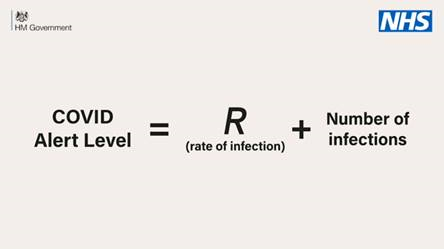
\includegraphics[width=0.48\textwidth]{images/r_plus}
        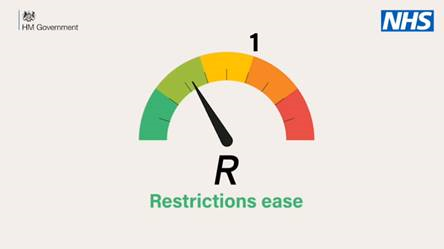
\includegraphics[width=0.48\textwidth]{images/r_dial}
        \caption{Government slides from coronavirus briefing, 10 May 2020}
        \label{gov-slides}
      \end{figure}
    }
    { % Solution
      Some obvious things here: it makes no sense to add $R_0$ to the number of infections, and the dial on the right suggests that there is a maximum and minimum $R_0$.
    }

    \question{The SIR model}
    { % Question
      We now move to the popular SIR disease model. This model separates the recovered population into a new group, $R$, assuming that they have become immune and therefore are no longer susceptible. The total population remains constant.

      \begin{enumerate}[label=(\alph*)]
        \item Write down equations for $\fd{S}{t}$, $\fd{I}{t}$, $\fd{R}{t}$ and $N$.
        \item So far, we haven't added birth and natural (non-epidemic) death to our model ($N$ has been constant). In what sort of situation might this be a reasonable choice?
        \item Given your equation for $N$, confirm that in your model, the total population is constant (i.e.\ that $\fd{N}{t} = 0$).
        \item Find all equilibria of the system. Is it/are they asymptotically stable? (Hint: pay close attention to our three possible cases at the end of section 2.2.)
        \item By combining two of your equations, find $S$ as a function of $R$ and hence demonstrate that this model predicts some individuals will always avoid infection if $S(0)>0$.
        \item Solutions for the infected population, $I$, either show monotonic decay or rise and have a peak infection value before decaying to the equilibrium $I=0$. Demonstrate that the criteria for the disease reaching a peak, i.e.\ that $I$ ever rises, is that
          \begin{equation}
            R_0>\frac{N}{S(0)}.
          \end{equation}
      \end{enumerate}
    }
    { % Solution
      \begin{enumerate}[label=(\alph*)]
        \item We have
          \begin{align}
            \fd{S}{t} &= - \beta I S, \\
            \fd{I}{t} &= \beta I S - \gamma I,\\
            \fd{R}{t} &= \gamma I, \\
            N &= S + I + R.
          \end{align}

        \item This choice is reasonable if the epidemic moves quite quickly.

        \item Adding the derivatives,
          \begin{equation}
            \fd{N}{t} = \fd{S}{t} + \fd{I}{t} + \fd{R}{t} = -\beta I S + \beta I S - \gamma I + \gamma I = 0.
          \end{equation}

        \item The equilibria ($\fd{S}{t} = \fd{I}{t} = \fd{R}{t} = 0$) only happen when $I=0$. In which case, $S = S_0$, frankly anything, and $R = N-S_0$. So we see there is a one-parameter family of equilibria, $(S_0,0,N-S_0)$, where  $S_0\in[0,N]$. It cannot be asymptotically stable as there is a nearby equilibrium always (it is a one-parameter family of equilibria). This is listed under the degenerate case in the notes.

        \item We divide the rate equations for $S$ and $R$ to obtain
          \begin{equation}
            \fd{S}{R} = \frac{-\beta S}{\gamma}.
          \end{equation}
          The solution is clearly an exponential,
          \begin{equation}
            S(t) = S(0)\e ^{-(\beta/\gamma)R} = S(0)\e ^{-R_0 R/N} \geq  S(0)\e ^{-R_0}.
          \end{equation}
          Now, since $R_0$ is a positive constant, $S(t)$ is bounded from below. The smaller $R_0$, the larger this bound is as a fraction of the initial population (which makes sense since smaller $R_0$ means people are recovering relatively quickly compared to the rate of infection).
        \item

          Take the equation for $I$, which can be written as
          \begin{equation}
            \fd{I}{t} = I[\beta S - \gamma].
          \end{equation}
          Note that, since $S$ is monotonically decreasing, the maximum value this rate can take is at $t=0$. Thus for the solution to rise we would need
          \begin{equation}
            \beta S(0) - \gamma > 0,
          \end{equation}
          giving the required condition.

      \end{enumerate}

    }

    %\section{Population dynamics SIR model}
    %Consider the following dynamic system for the development of a disease developing in a population $N(t)$. The population is split into three compartments: susceptible individuals, $S(t)$, infected individuals, $I(t)$, and recovered individuals, $R(t)$:
    %\begin{subequations}
    %\begin{align}
    %\fd{S}{t} &= -\frac{\beta I S}{N},\\
    %\fd{I}{t} &= \frac{\beta I S}{N}-\alpha I,\\
    %\fd{R}{t} &= \alpha I,\\
    %N&=S + I + R.
    %\end{align}
    %\end{subequations}
    %where $\alpha,\beta$ are positive real constants.
    %\begin{enumerate}[label=(\alph*)]
    %\item{Describe the interpretation of the terms on the right-hand side of the model.
    %}\item{
    %Demonstrate that the total population is constant.
    %}\item{
    %Find all equilibria of the system and assess if it/they are asymptotically stable.
    %}
    %\item{
    %Describe the physical interpretation of the so-called basic reproduction number $R_0= \beta/\alpha$.
    %}
    %\item{
    %Find $S$ as a function of $R$ and hence demonstrate that  this model predicts some individuals will always avoid infection if $S(0)>0$.
    %}\item{
    %Solutions for the infected population either show monotonic decay or rise and have a peak infection value before decaying to equilibrium $I=0$. Demonstrate that the criteria for the disease reaching a peak is that
    %\begin{equation}
    %R_0>N/S_0.
    %\end{equation}
    %}
    %\end{enumerate}
    %
    %Consider now the following extension of the basic SIR model, which includes both birth and death. This makes it more appropriate for the long term development of a disease:
    %\begin{subequations}
    %\begin{align}
    %\fd{S}{t} &=\mu(N-S) -\frac{\beta I S}{N},\\
    %\fd{I}{t} &= \frac{\beta I S}{N}-\alpha (I+\mu),\\
    %\fd{R}{t} &= \alpha I-\mu R,\\
    %N&=S + I + R,
    %\end{align}
    %\end{subequations}
    %where $\mu$ is the constant birth/death rate of the population.
    %
    %\begin{enumerate}[label=(\alph*),resume]
    %\item{Show, by solving the system rather than by direct substitution, that the following $(S,I,R)$ are the equilibria of the system:
    %\begin{equation}
    %(N,0,0),\quad \left(\frac{N}{R_0},\frac{\mu N(R_0-1)}{\beta},\frac{\alpha N(R_0-1)}{\beta}\right),
    %\end{equation}
    %where $R_0 =\beta/(\alpha +\mu)$ is again the basic reproduction number. The second equilibrium is the endemic equilibrium in which the diseases persists in the population, like influenza and likely Covid-19.
    %}\item{
    %Perform a linear stability analysis of these equilibria to show that if $R_0>1$ then the disease is endemic, and if $R_0<1$ it dies out.
    %}
    %\end{enumerate}

\end{enumerate}

\end{document}
